% 编译器：XeLaTeX
\documentclass[UTF8, 12pt]{ctexart}

% ===================== 页面与排版 =====================
\usepackage{geometry}
\geometry{
  a4paper,
  left=2.5cm, right=2.5cm,
  top=2.5cm,  bottom=2.5cm
}

% ===================== 数学 =====================
\usepackage{amsmath, amssymb, amsthm}
\newtheorem{theorem}{定理}[section]
\renewcommand{\proofname}{\textbf{证明}}

% ===================== 图表 =====================
\usepackage{graphicx}
\usepackage{float}
\usepackage{booktabs}
\usepackage{multirow}
\usepackage{caption}
\captionsetup{font=small, labelfont=bf}

% ===================== 代码高亮 =====================
\usepackage{tcolorbox}
\tcbuselibrary{listings, breakable}
\usepackage{listings}
\usepackage{xcolor}

\lstset{
  language=Python,
  basicstyle=\ttfamily\small,
  keywordstyle=\color{blue!80!black}\bfseries,
  commentstyle=\color{green!50!black}\itshape,
  stringstyle=\color{red!60!black},
  numbers=left,
  numberstyle=\tiny\color{gray},
  numbersep=6pt,
  breaklines=true,
  frame=none,
  showstringspaces=false,
  tabsize=4,
}

% ===================== 超链接 =====================
\usepackage{hyperref}
\hypersetup{
  colorlinks=true,
  linkcolor=blue!70!black,
  citecolor=green!50!black,
  urlcolor=cyan!60!black,
}

% ===================== 杂项 =====================
\usepackage{enumitem}

% ===================== 标题信息 =====================
\title{\textbf{Robust-PINN for Optimal Control Problems}\\[6pt]
       \large Scaling 策略的有效性验证与状态约束扩展}
\author{兰景琪\\[2pt] \small Mathematics 2026}
\date{}

% ==================================================================
\begin{document}
\maketitle

\tableofcontents
\newpage

% ==================================================================
\section{从优化问题到一阶最优性系统：(1.1)--(1.2) 向 (1.3) 的转化}
\label{sec:derivation}

对于带有约束条件的函数优化问题，可以理解为求目标函数在约束条件下的极值问题，即条件极值。
从数学分析的角度来说，即使用 Lagrange 乘数法。
PDE 约束下的问题同样可以采用 Lagrange 乘数法，核心思想不变——将有约束的问题转化为无约束问题。
先构造 Lagrange 函数：
\[
  L(x,\lambda) = f(x) + \lambda \cdot g(x),
\]
其中 $g(x)$ 为等式约束，$f(x)$ 为目标函数，$\lambda \cdot g(x)$ 称为\textbf{惩罚项}。
再利用变分原理，求解无约束问题的极值。

\subsection{Lagrange 函数的构造}

本问题的目标函数为：
\begin{equation}
  J(\bar{y}, \bar{u})
  = \frac{1}{2}\|\bar{y} - y_d\|_{L^2(\Omega)}^2
  + \frac{\alpha}{2}\|\bar{u} - u_d\|_{L^2(\Omega)}^2,
  \label{eq:objective}
\end{equation}
约束状态为：
\begin{equation}
  g(\bar{y}) = -\Delta\bar{y} - f - \bar{u} = 0.
  \label{eq:constraint}
\end{equation}
在函数空间 $L^2(\Omega)$ 中，"函数相乘"被内积量化，惩罚项为：
\begin{equation}
  \langle p,\, g(y)\rangle_{L^2(\Omega)}
  = \int_\Omega p(x)\bigl(-\Delta y(x) - f(x) - \bar{u}(x)\bigr)\,\mathrm{d}x.
  \label{eq:penalty-term}
\end{equation}

另外，PDE 约束 $-\Delta y - f - \bar{u} = 0$ 的解 $y$ 需满足正则性（光滑性）。
在偏微分方程理论中，椭圆型 PDE 的 Dirichlet 问题的解属于 $H_0^1(\Omega)$ 空间，即
\[
  H_0^1(\Omega) = \bigl\{v \in L^2(\Omega) \,\big|\, \nabla v \in L^2(\Omega;\mathbb{R}^d),\;
  v\big|_{\partial\Omega} = 0\bigr\}.
\]
$p$ 作为伴随状态，同样要求在 $\partial\Omega$ 上 $p=0$，便于后续分部积分。

\subsection{对状态 $\bar{y}$ 的变分}

根据变分原理，最优解需满足 Lagrange 函数对各变量的 Fréchet 导数为零。

\paragraph{第一部分——目标函数对 $\bar{y}$ 的变分：}
\[
  \frac{\delta J}{\delta\bar{y}}
  = \frac{\partial}{\partial\bar{y}}\!\left(\frac{1}{2}\int_\Omega(\bar{y}-y_d)^2\,\mathrm{d}x\right)
  = \int_\Omega(\bar{y}-y_d)\,\delta\bar{y}\,\mathrm{d}x
  = \langle\bar{y}-y_d,\;\delta\bar{y}\rangle_{L^2}.
\]

\paragraph{第二部分——惩罚项对 $\bar{y}$ 的变分：}
利用 Green 第一公式：对任意 $u,v\in H_0^1(\Omega)$（边界上 $u=v=0$），有
\begin{equation}
  \int_\Omega \nabla u \cdot \nabla v\,\mathrm{d}x
  = -\int_\Omega v\,\Delta u\,\mathrm{d}x
  + \underbrace{\int_{\partial\Omega} v\,\nabla u \cdot \mathbf{n}\,\mathrm{d}S}_{\text{边界项}}.
  \label{eq:green}
\end{equation}
由于 $p$ 和 $\delta\bar{y}$ 在 $\partial\Omega$ 上均为零，边界项消失，因此
\[
  \int_\Omega p\,(-\Delta\delta\bar{y})\,\mathrm{d}x
  = \int_\Omega \delta\bar{y}\,(-\Delta p)\,\mathrm{d}x,
  \qquad\text{即}\quad
  \langle p,\,-\Delta\delta\bar{y}\rangle_{L^2}
  = \langle -\Delta p,\,\delta\bar{y}\rangle_{L^2}.
\]

\paragraph{合并：} 变分条件为
\[
  \delta\mathcal{L}
  = \langle\bar{y}-y_d,\;\delta\bar{y}\rangle_{L^2}
  + \langle -\Delta p,\;\delta\bar{y}\rangle_{L^2}
  = \langle\bar{y}-y_d - \Delta p,\;\delta\bar{y}\rangle_{L^2}
  = 0,
  \quad\forall\,\delta\bar{y}.
\]
由 $L^2$ 内积的非退化性，被积函数必须为零，从而得伴随方程：
\begin{equation}
  \boxed{-\Delta p = -(\ \bar{y} - y_d).}
  \label{eq:adjoint}
\end{equation}

\subsection{对控制 $\bar{u}$ 的变分}

目标函数对 $\bar{u}$ 的梯度为 $\langle\alpha(\bar{u}-u_d),\,\delta\bar{u}\rangle_{L^2}$，
惩罚项对 $\bar{u}$ 的梯度为 $-\langle p,\,\delta\bar{u}\rangle_{L^2}$。
合并得：
\[
  \langle\alpha(\bar{u}-u_d) - p,\;\delta\bar{u}\rangle_{L^2} = 0
  \quad\forall\,\delta\bar{u},
\]
从而
\begin{equation}
  p = \alpha(\bar{u} - u_d).
  \label{eq:control-eq}
\end{equation}

\begin{tcolorbox}[colback=blue!5!white, colframe=blue!60!black, title={注}]
如果问题的 Lagrange 函数定义为
$\mathcal{L}(y,u;p) = J(y,u) + \int_\Omega(\Delta y + f + u)\,p\,\mathrm{d}x$，
则一阶最优性系统为
\begin{equation}
  \begin{cases}
    -\Delta\bar{y} = f + \bar{u}  &\text{in } \Omega,\quad \bar{y}=0 \text{ on } \partial\Omega,\\
    -\Delta\bar{p} = \bar{y}-y_d  &\text{in } \Omega,\quad \bar{p}=0 \text{ on } \partial\Omega,\\
    \alpha(\bar{u}-u_d)+\bar{p}=0.
  \end{cases}
  \label{eq:kkt-alt}
\end{equation}
\end{tcolorbox}

\subsection{对伴随 $p$ 的变分}

Lagrange 函数中与 $p$ 相关的项仅为
$\langle p,\,-\Delta\bar{y}-f-\bar{u}\rangle_{L^2}$，
对 $p$ 求变分得：
\[
  \langle -\Delta\bar{y}-f-\bar{u},\;\delta p\rangle_{L^2} = 0
  \quad\forall\,\delta p,
\]
即得状态方程：
\begin{equation}
  \boxed{-\Delta\bar{y} = f + \bar{u} \quad\text{in } \Omega, \qquad \bar{y}=0 \quad\text{on } \partial\Omega.}
  \label{eq:state}
\end{equation}


% ==================================================================
\section{Scaling 处理对敏感性降低的有效性}
\label{sec:scaling-effectiveness}

% ============================================================
% 插入位置：scailing_report.tex 中 \section{Scaling 处理对敏感性降低的有效性}
%           \label{sec:scaling-effectiveness} 之后
% ============================================================

本节通过系统性的数值实验，验证 (1.5) 式 Scaling 变换对 PINN 求解椭圆最优控制问题时
降低参数敏感性的有效性。实验从两个维度展开：
\begin{itemize}
  \item \textbf{$\alpha$-敏感性}：固定损失函数权重，验证 Scaling 后误差对正则化参数
        $\alpha$ 的变化不敏感；
  \item \textbf{$\omega$-敏感性}：固定 $\alpha$ 于病态值 $10^{-4}$，验证 Scaling 后误差对
        损失函数全局权重 $\omega$ 的变化不敏感。
\end{itemize}
每种维度下分别在不同网络架构（Unified Network / Dual Network）和边界条件处理方式
（Hard BC / Soft BC）下进行对照实验，共计 6 组实验。


% ==================================================================
\subsection{实验设置}
\label{subsec:exp-setup}

\paragraph{精确解构造（MMS）。}
在 $\Omega = [0,1]^2$ 上取齐次 Dirichlet 边界条件，构造精确解
\[
  \bar{y}(x) = \sin(\pi x_1)\sin(\pi x_2), \qquad
  \bar{p}(x) = \alpha\sin(\pi x_1)\sin(\pi x_2).
\]
由最优性系统 (1.3) 反推源项及目标函数
\[
  f(x) = (2\pi^2 + 1)\,\bar{y}(x), \qquad
  y_d(x) = (1 - 2\pi^2\alpha)\,\bar{y}(x), \qquad
  u_d \equiv 0,
\]
以确保可精确定量验证。

\paragraph{网络架构。}
\begin{itemize}
  \item \textbf{Unified Network}（单网络双输出）：3 层隐藏层，每层 50 个神经元，
        SiLU 激活函数，输出维度为 2，分别表示 $y$ 和 $p$；
  \item \textbf{Dual Network}（双独立网络）：$y$ 和 $p$ 各由一个独立的同结构网络拟合，
        输出维度为 1。
\end{itemize}

\paragraph{边界条件处理。}
\begin{itemize}
  \item \textbf{硬边界（Hard BC）}：采用距离函数 Ansatz
        $\hat{y}(x) = D(x)\cdot N_\theta(x)$，
        其中 $D(x) = x_1(1-x_1)\,x_2(1-x_2)$，自动精确满足齐次 Dirichlet 边界条件；
  \item \textbf{软边界（Soft BC）}：不使用距离函数，将边界条件作为惩罚项加入损失函数
        $\mathcal{L} = \mathcal{L}_{\mathrm{PDE}} + w_{\mathrm{bc}}\,\mathcal{L}_{\mathrm{BC}}$。
\end{itemize}

\paragraph{Scaling 实现细节。}
未缩放系统直接求解 (1.4) 式，网络输出即为物理量 $\bar{y},\bar{p}$。
缩放系统求解 (1.5) 式：网络的原始输出 $N_y, N_p$ 经特征尺度放缩映射为缩放变量
$y = \alpha^{1/4}\,N_y$，$p = \alpha^{3/4}\,N_p$；
评估误差时通过逆变换 $\bar{y} = \alpha^{-1/4}\,y$，$\bar{p} = \alpha^{1/4}\,p$
恢复物理量。
此外，在计算缩放系统的损失时，对残差逐项除以对应特征尺度
（$R_1/\alpha^{3/4}$，$R_2/\alpha^{1/4}$）进行归一化，消除残差之间的量级差异。

\paragraph{训练策略。}
采用 Adam + L-BFGS 混合训练：先用 Adam（$\mathrm{lr}=10^{-3}$）训练 1500 个 epoch
进行全局探索，再用 L-BFGS（strong Wolfe 线搜索，最多 1000 次迭代）进行高精度局部收敛。
内部配点 2500 个（均匀随机采样），边界配点 400 个（每边 100 个，仅 Soft BC 使用）。

\paragraph{误差度量。}
对 $\bar{y}$ 和 $\bar{p}$ 分别报告三种误差范数：
相对 $L^2$ 误差 $e_{L^2} = \|u - u_h\|_{L^2}\big/\|u\|_{L^2}$，
$L^\infty$ 误差（最大绝对误差）$e_\infty = \max|u - u_h|$，
以及相对 $H^1$ 误差 $e_{H^1} = \|u - u_h\|_{H^1}\big/\|u\|_{H^1}$。
其中表格仅列出 $L^2$ 与 $H^1$ 误差，$L^\infty$ 结果可在对应图中查阅。


% ==================================================================
\subsection{$\alpha$-敏感性实验}
\label{subsec:alpha-test}

固定损失函数权重为等权重（$w_1 = w_2 = 1$），在
$\alpha \in \{10^{-2},\,10^{-3},\,10^{-4},\,10^{-5}\}$
（部分实验扩展至 $\alpha = 1$）上对比 Unscaled 与 Scaled 系统的求解精度。

% ------------------------------------------------------------------
\subsubsection{Hard BC + Unified Network（基准实验）}

硬边界条件下单网络双输出架构的实验结果见表~\ref{tab:alpha-hard-unified}。

\begin{table}[H]
  \centering
  \caption{$\alpha$-敏感性实验：Hard BC + Unified Network}
  \label{tab:alpha-hard-unified}
  \small
  \begin{tabular}{cc rrrr}
    \toprule
    $\alpha$ & 系统 & $L^2_y$ & $L^2_p$ & $H^1_y$ & $H^1_p$ \\
    \midrule
    \multirow{2}{*}{$10^{-2}$}
      & Unscaled & $5.06\times10^{-5}$ & $3.01\times10^{-3}$
                 & $1.27\times10^{-4}$ & $7.50\times10^{-3}$ \\
      & Scaled   & $7.15\times10^{-5}$ & $3.03\times10^{-3}$
                 & $1.34\times10^{-4}$ & $4.87\times10^{-3}$ \\
    \midrule
    \multirow{2}{*}{$10^{-3}$}
      & Unscaled & $7.77\times10^{-4}$ & $5.75\times10^{-2}$
                 & $1.43\times10^{-3}$ & $1.49\times10^{-1}$ \\
      & Scaled   & $3.06\times10^{-4}$ & $8.09\times10^{-3}$
                 & $3.44\times10^{-4}$ & $1.09\times10^{-2}$ \\
    \midrule
    \multirow{2}{*}{$10^{-4}$}
      & Unscaled & $9.32\times10^{-1}$ & $1.84\times10^{+1}$
                 & $9.32\times10^{-1}$ & $1.84\times10^{+1}$ \\
      & Scaled   & $6.85\times10^{-4}$ & $1.37\times10^{-2}$
                 & $6.95\times10^{-4}$ & $1.43\times10^{-2}$ \\
    \midrule
    \multirow{2}{*}{$10^{-5}$}
      & Unscaled & $9.94\times10^{-1}$ & $1.96\times10^{+1}$
                 & $9.94\times10^{-1}$ & $1.96\times10^{+1}$ \\
      & Scaled   & $1.09\times10^{-3}$ & $2.17\times10^{-2}$
                 & $1.10\times10^{-3}$ & $2.20\times10^{-2}$ \\
    \bottomrule
  \end{tabular}
\end{table}

Unscaled 系统在 $\alpha \leq 10^{-4}$ 时完全失效，相对 $L^2$ 误差趋近~1
（即网络输出近似为零），这与定理~\ref{thm:gradient-divergence} 的梯度爆炸预测一致。
Scaled 系统在全部 $\alpha$ 范围内保持 $L^2_y \sim 10^{-4}$--$10^{-3}$、
$L^2_p \sim 10^{-3}$--$10^{-2}$，误差量级跨 $\alpha$ 变化极为稳定
（图~\ref{fig:alpha-hard-unified}）。

\begin{figure}[H]
  \centering
  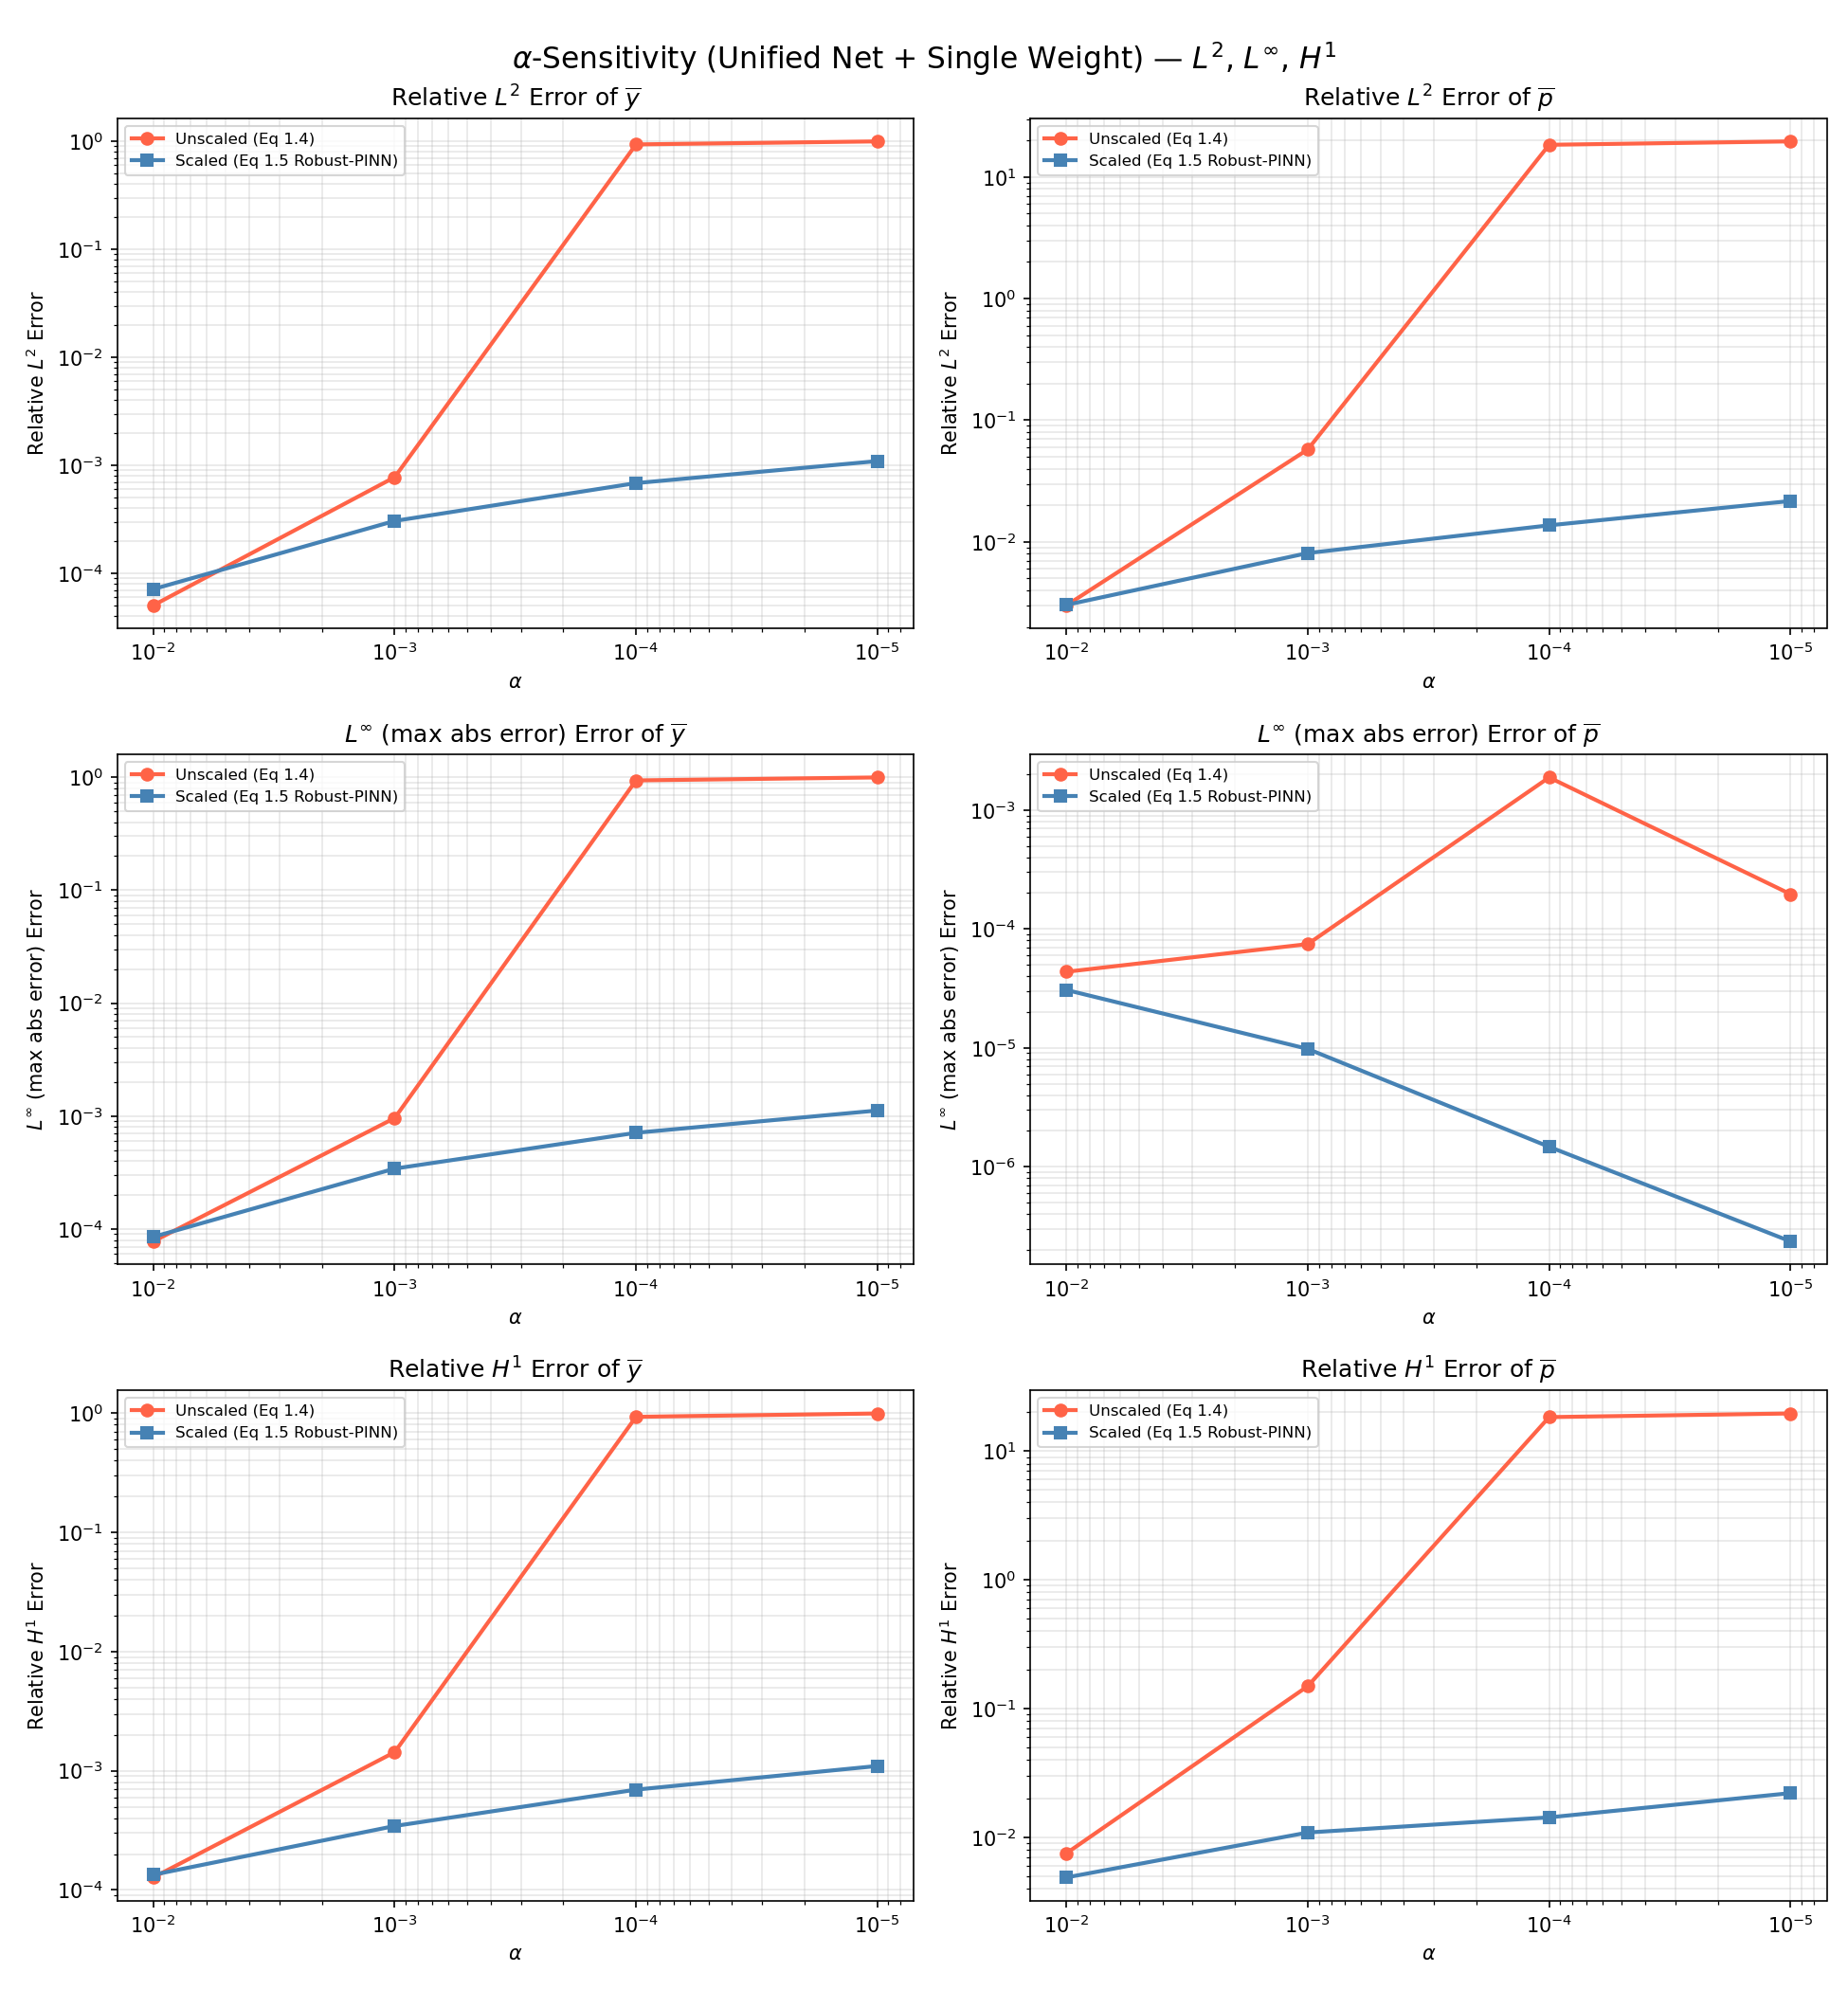
\includegraphics[width=\linewidth]{alpha_test_hardBC/unified_sensitivity_result.png}
  \caption{$\alpha$-敏感性（Hard BC + Unified Network）：
           $L^2$、$L^\infty$、$H^1$ 误差随 $\alpha$ 的变化}
  \label{fig:alpha-hard-unified}
\end{figure}


% ------------------------------------------------------------------
\subsubsection{Soft BC + Dual Network}

移除距离函数 Ansatz，改用软边界惩罚（$w_{\mathrm{bc}} = 100$），
并在 Scaled 系统中对边界残差同样除以特征尺度进行归一化。
结果见表~\ref{tab:alpha-soft-dual}。

\begin{table}[H]
  \centering
  \caption{$\alpha$-敏感性实验：Soft BC + Dual Network（$w_{\mathrm{bc}}=100$）}
  \label{tab:alpha-soft-dual}
  \small
  \begin{tabular}{cc rrrr}
    \toprule
    $\alpha$ & 系统 & $L^2_y$ & $L^2_p$ & $H^1_y$ & $H^1_p$ \\
    \midrule
    \multirow{2}{*}{$10^{-2}$}
      & Unscaled & $1.49\times10^{-3}$ & $1.35\times10^{-1}$
                 & $2.84\times10^{-3}$ & $2.63\times10^{-1}$ \\
      & Scaled   & $4.82\times10^{-2}$ & $9.96\times10^{-1}$
                 & $4.98\times10^{-2}$ & $9.96\times10^{-1}$ \\
    \midrule
    \multirow{2}{*}{$10^{-3}$}
      & Unscaled & $8.82\times10^{-1}$ & $1.77\times10^{+1}$
                 & $8.98\times10^{-1}$ & $1.91\times10^{+1}$ \\
      & Scaled   & $5.00\times10^{-2}$ & $1.00\times10^{+0}$
                 & $5.05\times10^{-2}$ & $1.00\times10^{+0}$ \\
    \midrule
    \multirow{2}{*}{$10^{-4}$}
      & Unscaled & $9.89\times10^{-1}$ & $1.94\times10^{+1}$
                 & $1.00\times10^{+0}$ & $1.94\times10^{+1}$ \\
      & Scaled   & $5.01\times10^{-2}$ & $9.99\times10^{-1}$
                 & $5.05\times10^{-2}$ & $9.99\times10^{-1}$ \\
    \midrule
    \multirow{2}{*}{$10^{-5}$}
      & Unscaled & $9.96\times10^{-1}$ & $1.95\times10^{+1}$
                 & $1.00\times10^{+0}$ & $1.96\times10^{+1}$ \\
      & Scaled   & $5.01\times10^{-2}$ & $9.99\times10^{-1}$
                 & $5.05\times10^{-2}$ & $9.99\times10^{-1}$ \\
    \bottomrule
  \end{tabular}
\end{table}

Scaled 系统对 $\bar{y}$ 的拟合显著优于 Unscaled（$L^2_y \sim 0.05$ vs.\ $\sim 1.0$），
但伴随状态 $\bar{p}$ 的相对 $L^2$ 误差 $\approx 1.0$。
这并非 Scaling 失效：$\bar{p} = \alpha\sin(\pi x_1)\sin(\pi x_2)$ 在小 $\alpha$ 下
量值极小（$\sim\!\mathcal{O}(\alpha)$），极小的绝对偏差即导致极大的相对误差。
事实上其最大绝对误差 $L^\infty_p \sim \mathcal{O}(\alpha)$
（如 $\alpha=10^{-4}$ 时 $L^\infty_p = 9.99\times10^{-5}$），
说明 $\bar{p}$ 的绝对预测精度仍合理。
双独立网络缺乏参数共享的隐式耦合，在软边界下难以同时精确拟合两个量级差异悬殊的变量，
是导致该现象的根本原因。

\begin{figure}[H]
  \centering
  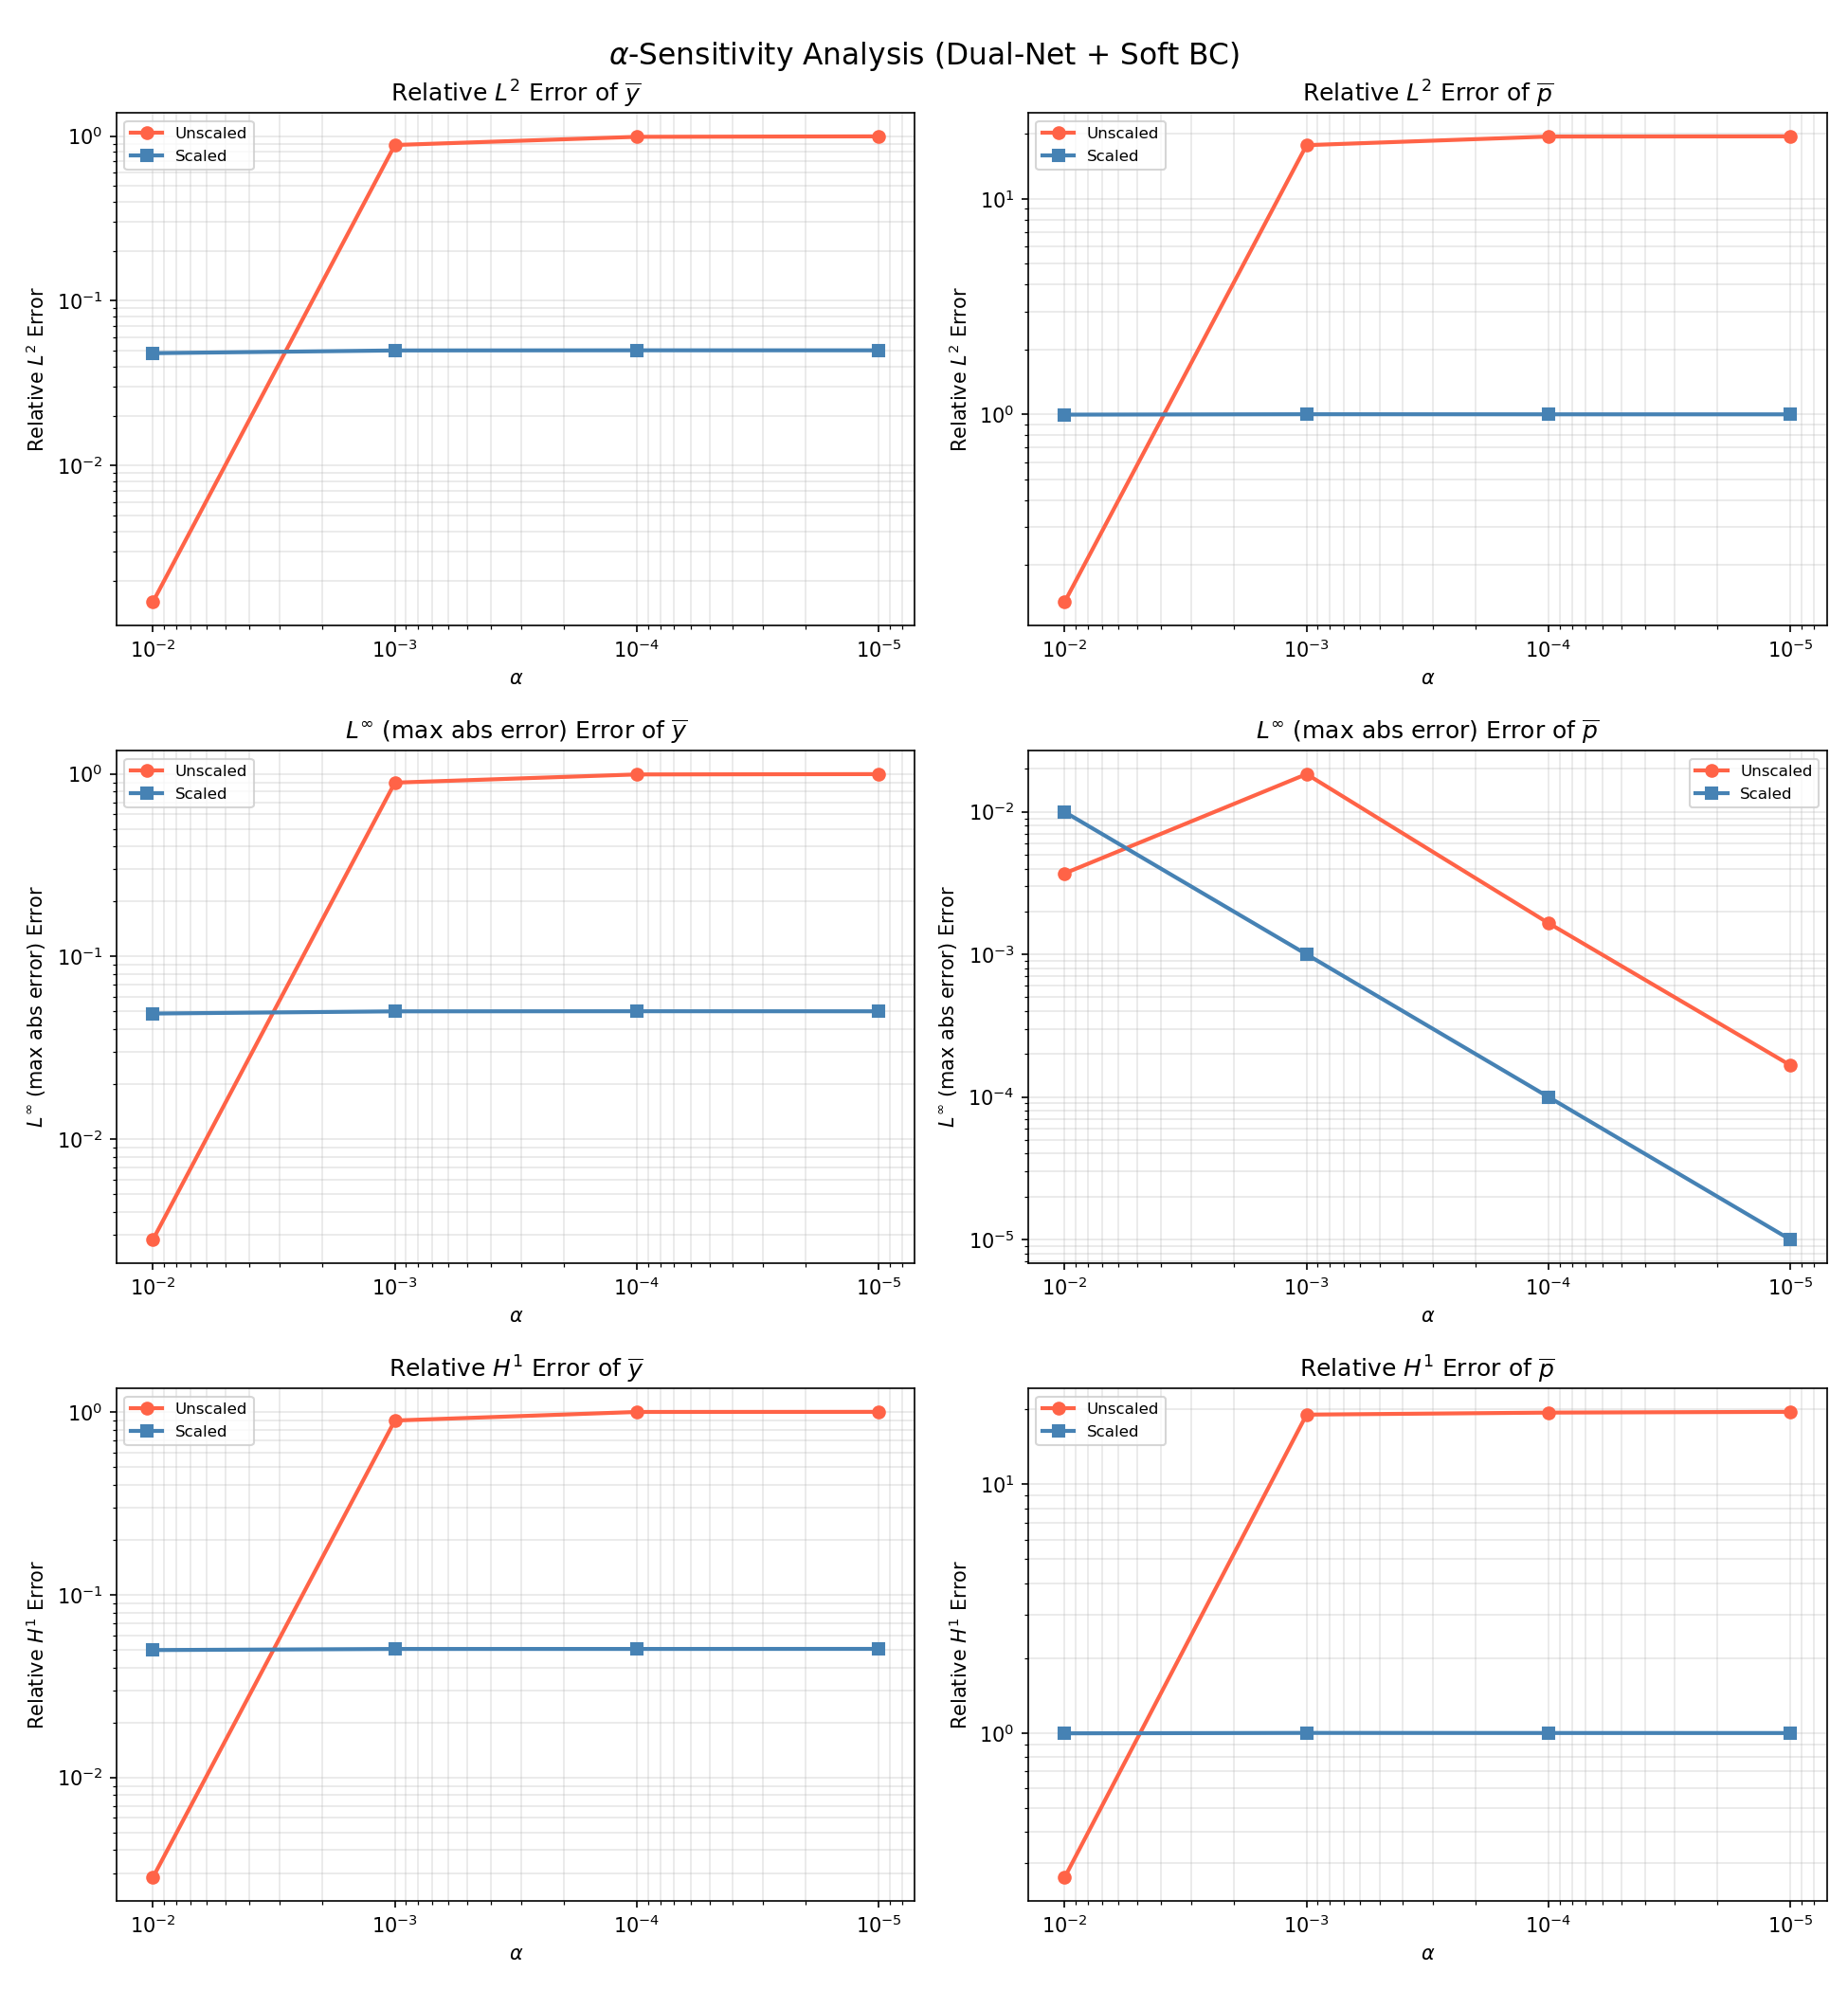
\includegraphics[width=\linewidth]{alpha_test_softBC_dualnet/dual_net_soft_bc_result.png}
  \caption{$\alpha$-敏感性（Soft BC + Dual Network，$w_{\mathrm{bc}}=100$）：
           $L^2$、$L^\infty$、$H^1$ 误差随 $\alpha$ 的变化}
  \label{fig:alpha-soft-dual}
\end{figure}

作为补充，将边界惩罚权重降至 $w_{\mathrm{bc}} = 1$（等权重）的对照实验
（图~\ref{fig:alpha-soft-dual-eq}）表明趋势一致，但整体精度略有下降，
说明在软边界设置中适当提高 $w_{\mathrm{bc}}$ 有助于改善求解质量。

\begin{figure}[H]
  \centering
  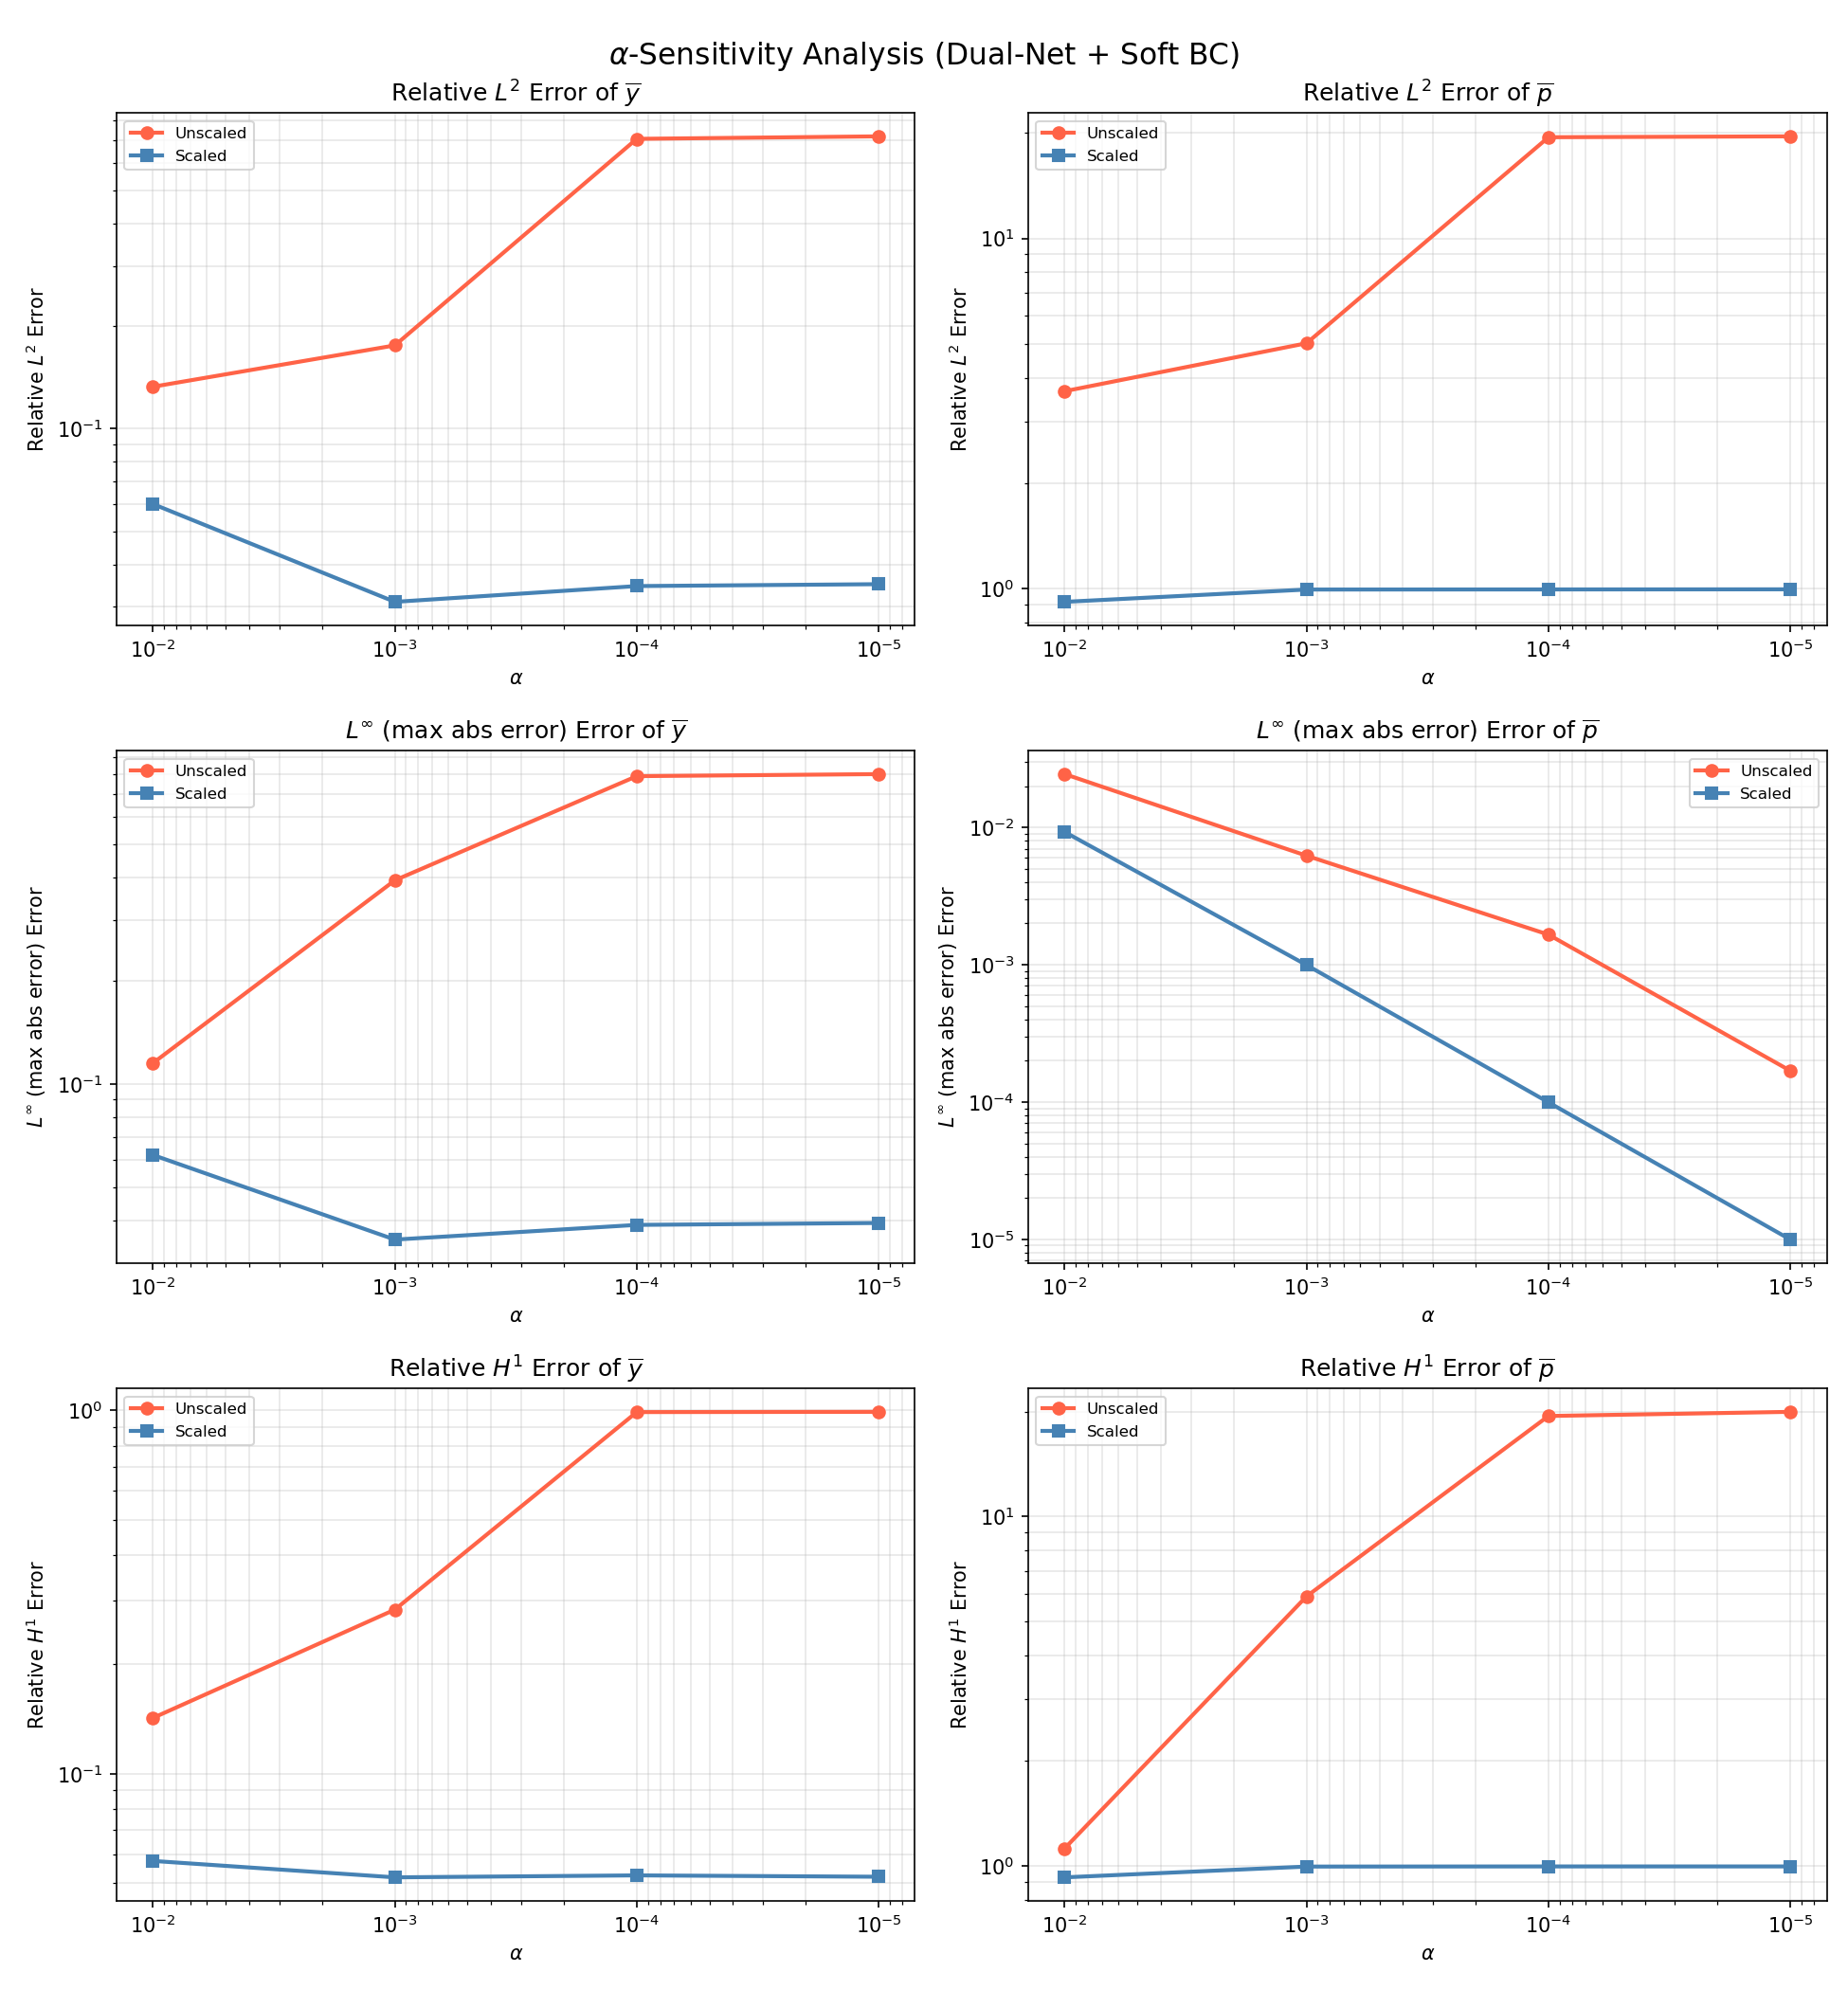
\includegraphics[width=\linewidth]{alpha_test_softBC_dualnet/dual_net_soft_bc_result_equweight.png}
  \caption{Soft BC + Dual Network（等权重 $w_{\mathrm{bc}}=1$）的 $\alpha$-敏感性对照}
  \label{fig:alpha-soft-dual-eq}
\end{figure}


% ------------------------------------------------------------------
\subsubsection{Soft BC + Unified Network}

将网络架构切换为单网络双输出（参数共享），边界惩罚权重提升至 $w_{\mathrm{bc}} = 1000$，
$\alpha$ 的扫描范围扩展至 $\{1,\,10^{-1},\,10^{-2},\,10^{-3},\,10^{-4},\,10^{-5}\}$。

\begin{table}[H]
  \centering
  \caption{$\alpha$-敏感性实验：Soft BC + Unified Network（$w_{\mathrm{bc}}=1000$）}
  \label{tab:alpha-soft-unified}
  \small
  \begin{tabular}{cc rrrr}
    \toprule
    $\alpha$ & 系统 & $L^2_y$ & $L^2_p$ & $H^1_y$ & $H^1_p$ \\
    \midrule
    \multirow{2}{*}{$1$}
      & Unscaled & $3.57\times10^{-3}$ & $3.99\times10^{-3}$
                 & $9.72\times10^{-3}$ & $1.09\times10^{-2}$ \\
      & Scaled   & $3.81\times10^{-3}$ & $3.57\times10^{-3}$
                 & $9.23\times10^{-3}$ & $1.00\times10^{-2}$ \\
    \midrule
    \multirow{2}{*}{$10^{-1}$}
      & Unscaled & $3.45\times10^{-3}$ & $1.33\times10^{-2}$
                 & $9.69\times10^{-3}$ & $2.07\times10^{-2}$ \\
      & Scaled   & $2.51\times10^{-3}$ & $2.38\times10^{-3}$
                 & $5.37\times10^{-3}$ & $5.62\times10^{-3}$ \\
    \midrule
    \multirow{2}{*}{$10^{-2}$}
      & Unscaled & $8.39\times10^{-2}$ & $2.34\times10^{+0}$
                 & $9.23\times10^{-2}$ & $8.21\times10^{-1}$ \\
      & Scaled   & $2.15\times10^{-3}$ & $6.20\times10^{-3}$
                 & $5.35\times10^{-3}$ & $1.21\times10^{-2}$ \\
    \midrule
    \multirow{2}{*}{$10^{-3}$}
      & Unscaled & $6.00\times10^{-1}$ & $1.89\times10^{+1}$
                 & $9.54\times10^{-1}$ & $1.95\times10^{+1}$ \\
      & Scaled   & $5.79\times10^{-3}$ & $1.90\times10^{-1}$
                 & $1.12\times10^{-2}$ & $1.91\times10^{-1}$ \\
    \midrule
    \multirow{2}{*}{$10^{-4}$}
      & Unscaled & $7.03\times10^{-1}$ & $1.95\times10^{+1}$
                 & $9.86\times10^{-1}$ & $1.97\times10^{+1}$ \\
      & Scaled   & $7.23\times10^{-3}$ & $2.18\times10^{-1}$
                 & $1.27\times10^{-2}$ & $2.19\times10^{-1}$ \\
    \midrule
    \multirow{2}{*}{$10^{-5}$}
      & Unscaled & $7.15\times10^{-1}$ & $1.96\times10^{+1}$
                 & $9.87\times10^{-1}$ & $2.02\times10^{+1}$ \\
      & Scaled   & $8.81\times10^{-3}$ & $2.61\times10^{-1}$
                 & $1.41\times10^{-2}$ & $2.63\times10^{-1}$ \\
    \bottomrule
  \end{tabular}
\end{table}

\begin{figure}[H]
  \centering
  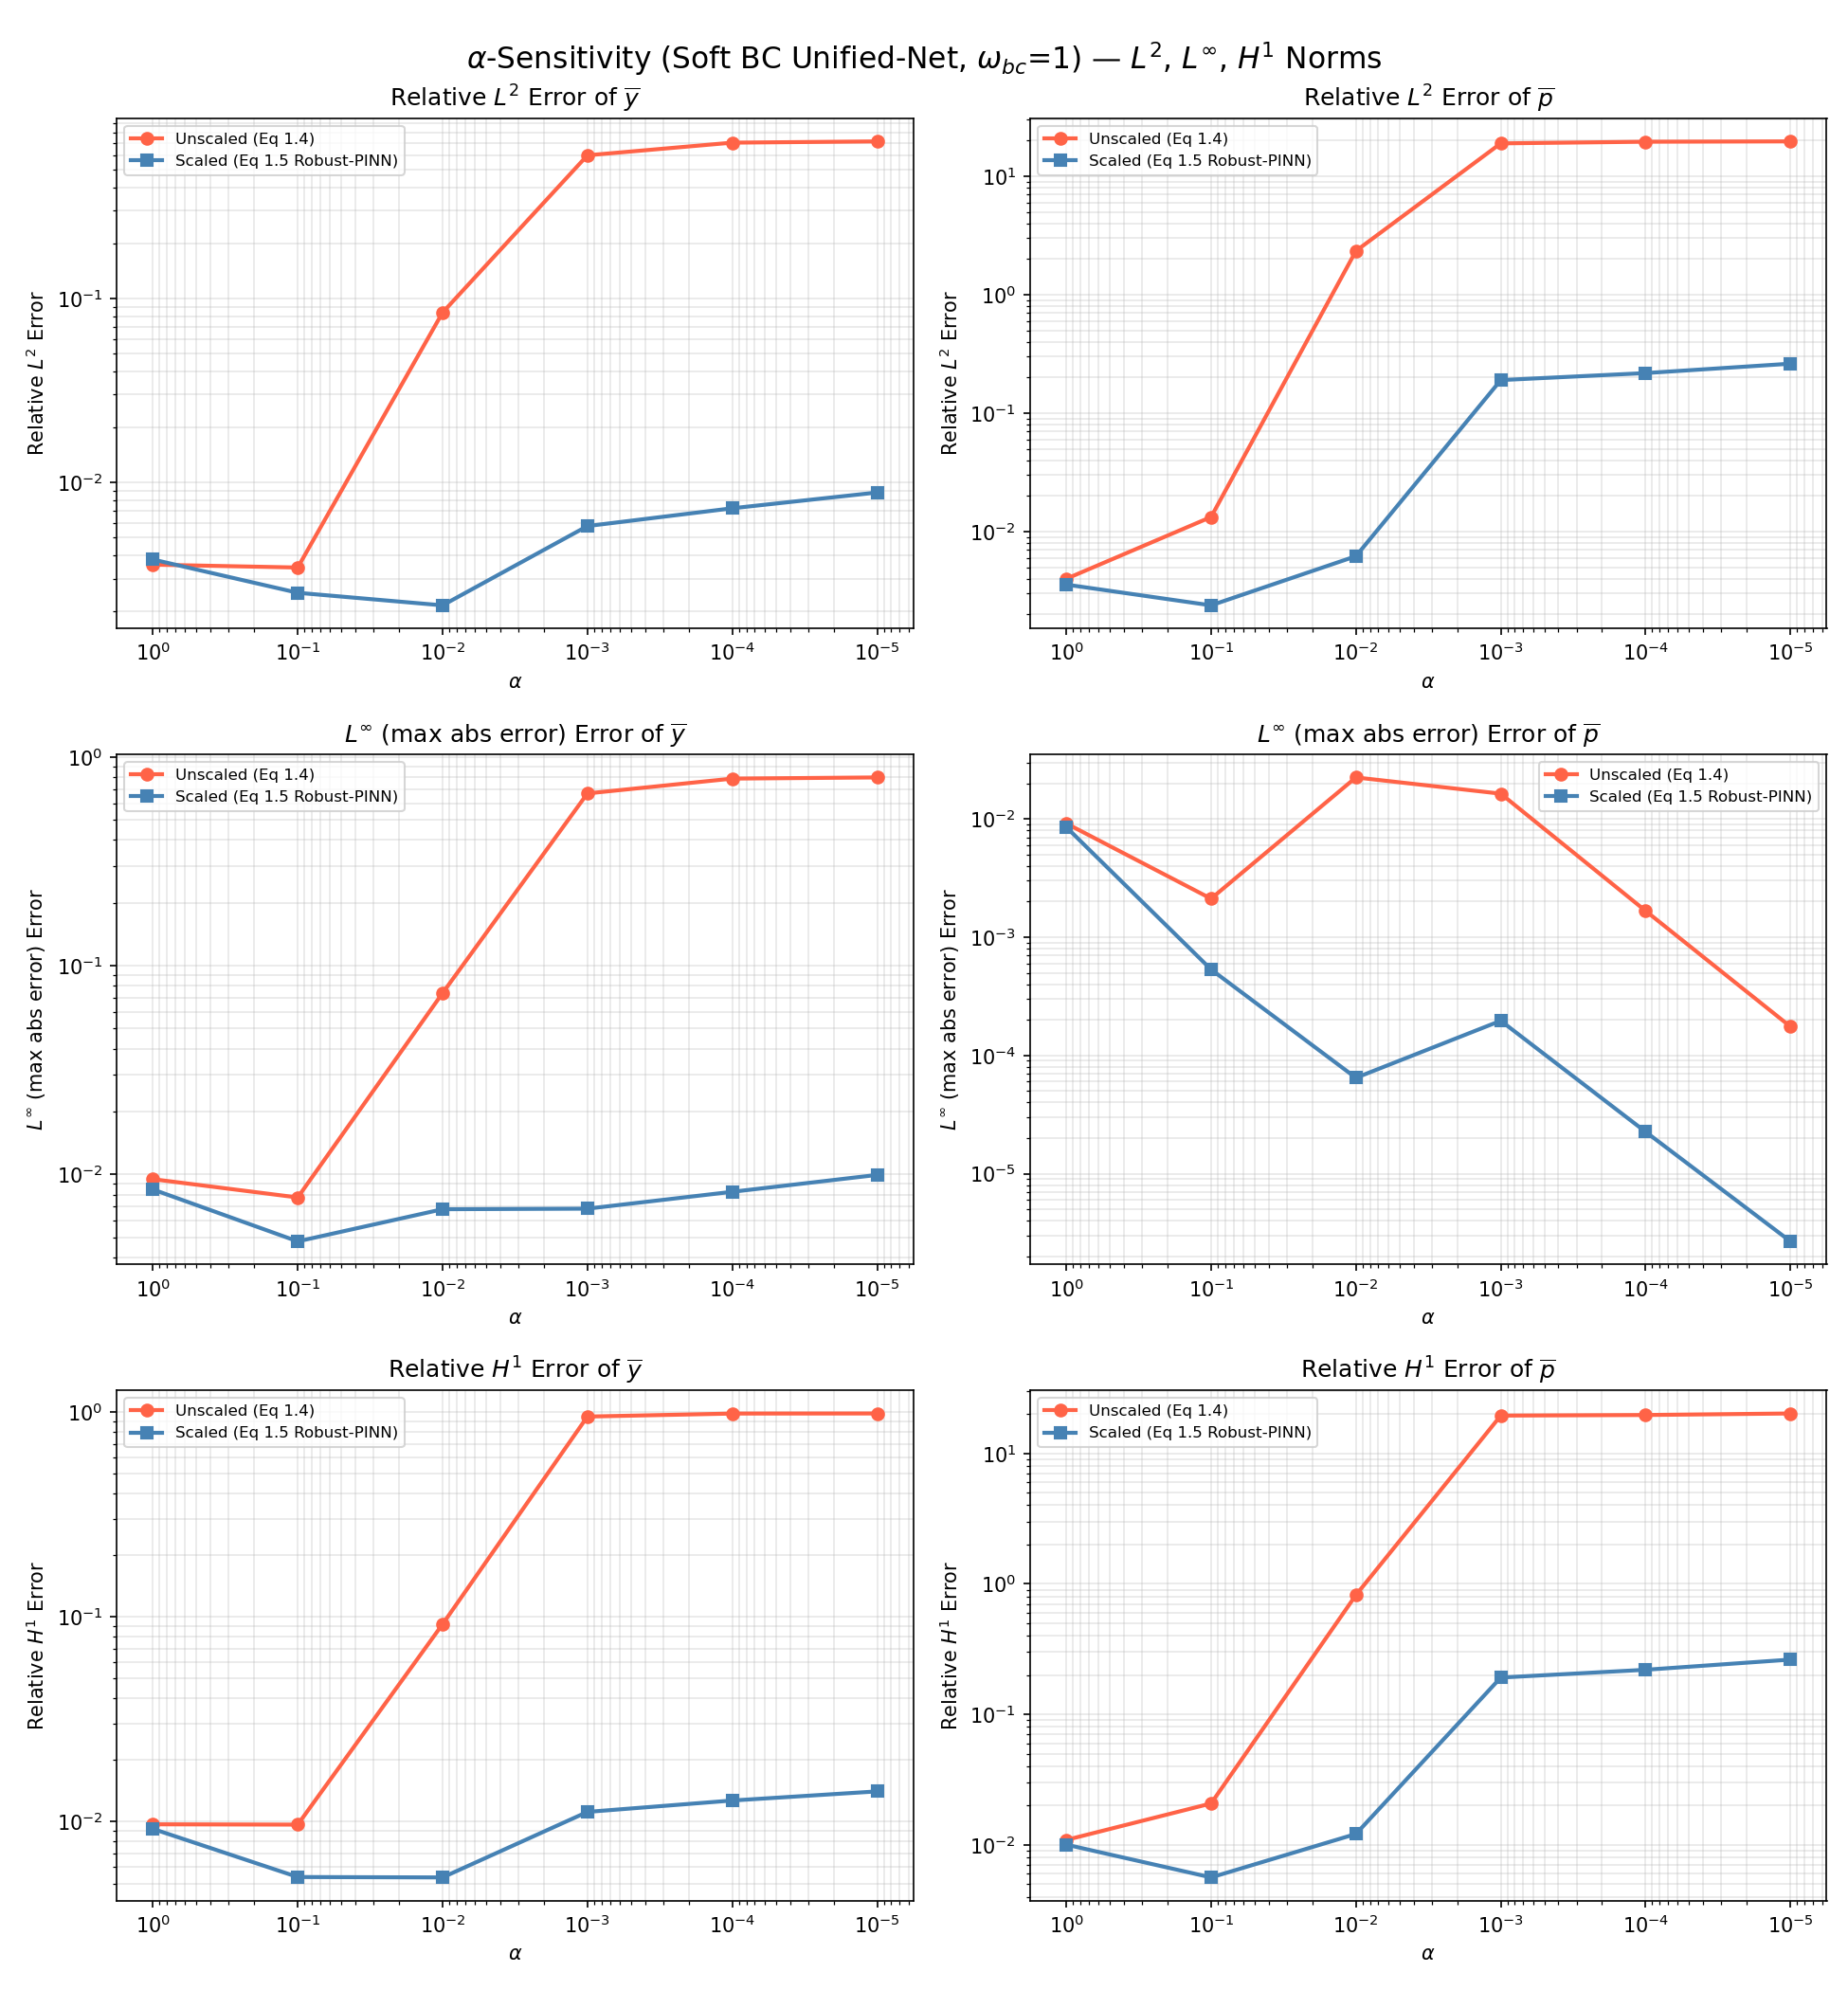
\includegraphics[width=\linewidth]{alpha_test_softBC_unified/alpha_test_softBC_unified_result1.png}
  \caption{$\alpha$-敏感性（Soft BC + Unified Network，$w_{\mathrm{bc}}=1000$）：
           $L^2$、$L^\infty$、$H^1$ 误差随 $\alpha$ 的变化}
  \label{fig:alpha-soft-unified}
\end{figure}

相比 Dual Network，Unified Network 在 Soft BC 下的表现显著改善：
Scaled 系统的 $L^2_y$ 在整个 $\alpha$ 范围内稳定在 $10^{-3}$ 量级；
$L^2_p$ 降至 $\sim\!0.2$（Dual Network 下为 $\sim\!1.0$），
说明参数共享引入的隐式耦合有助于伴随状态的协同学习。
当 $\alpha \geq 10^{-2}$ 时，Scaled 的 $L^2_p$ 可降至 $10^{-3}$ 量级，
与 Hard BC 精度接近。

此外，将边界惩罚改为等权重 $w_{\mathrm{bc}} = 1$
（图~\ref{fig:alpha-soft-unified-sw}）后，
Scaled 系统的 $L^2_y$ 同样保持在 $10^{-3}$--$10^{-2}$ 量级，
进一步证实 Scaling 的鲁棒性不依赖于特定的 $w_{\mathrm{bc}}$ 取值。

\begin{figure}[H]
  \centering
  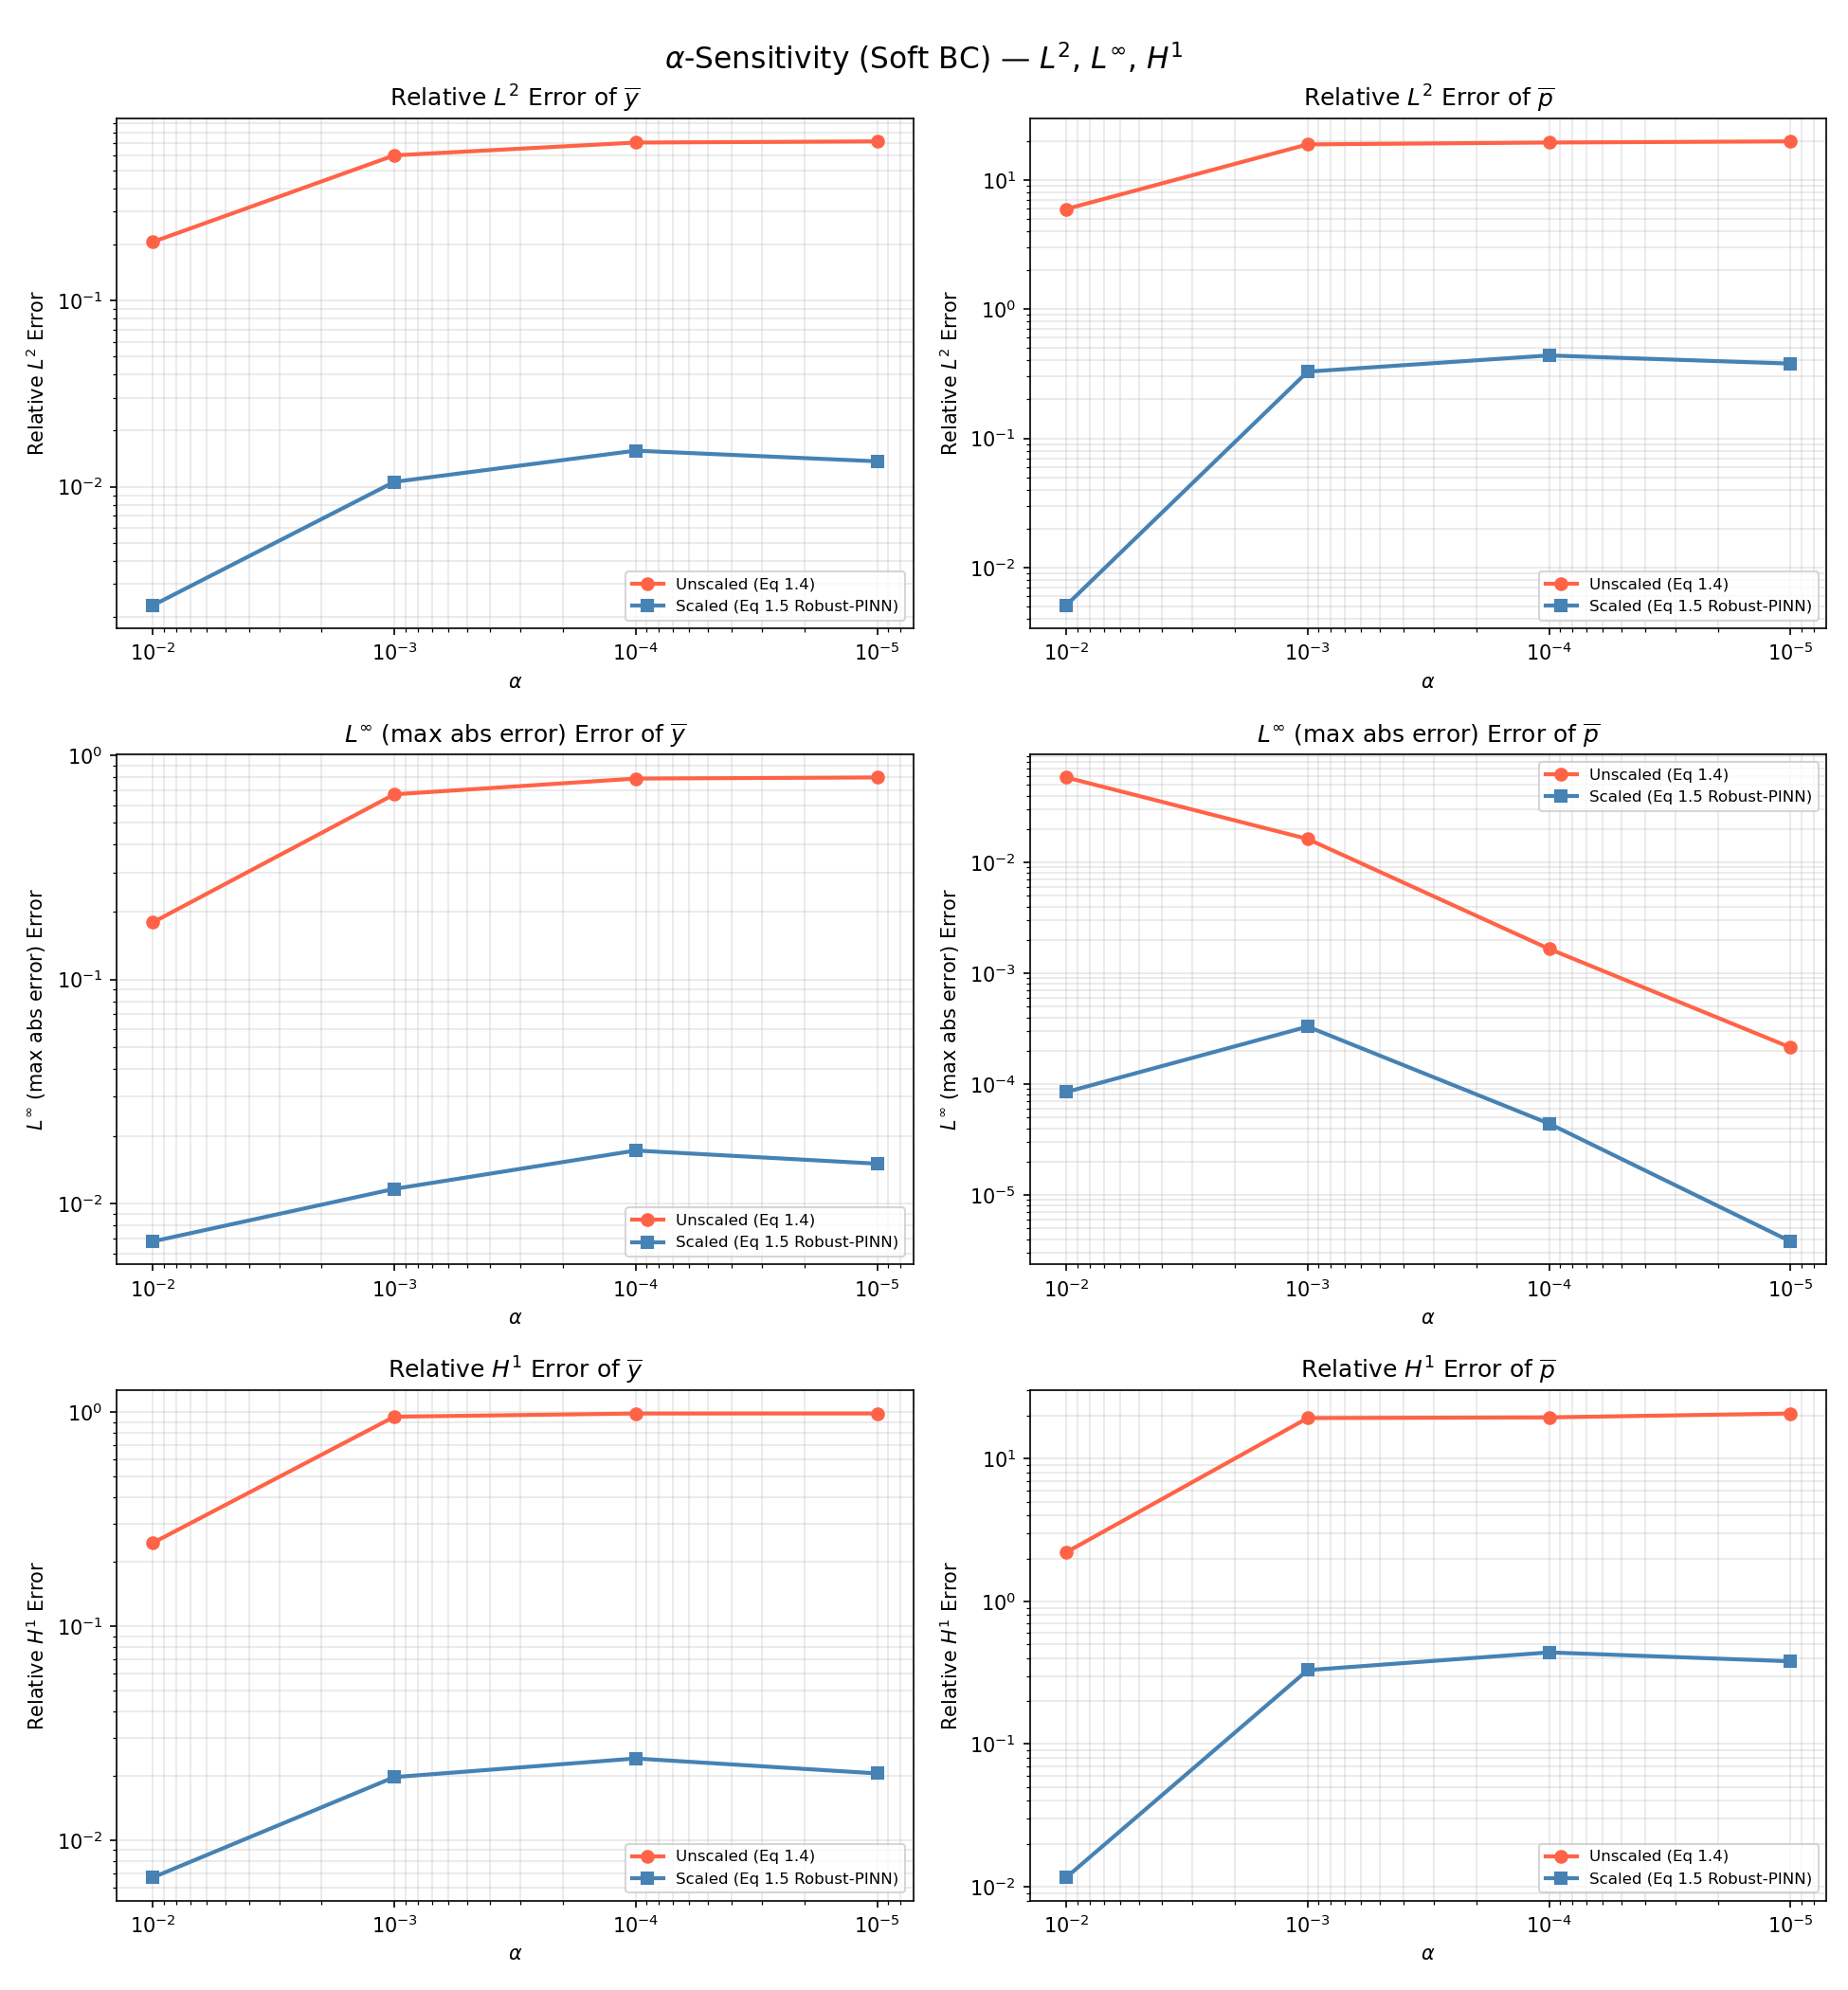
\includegraphics[width=\linewidth]{alpha_test_softBC_unified/unified_sensitivity_soft_bc_result_sameweight.png}
  \caption{Soft BC + Unified Network（等权重 $w_{\mathrm{bc}}=1$）的
           $\alpha$-敏感性对照}
  \label{fig:alpha-soft-unified-sw}
\end{figure}


% ------------------------------------------------------------------
\subsubsection{$\alpha$-敏感性实验小结}

三组实验一致表明：
\begin{enumerate}
  \item Unscaled 系统在 $\alpha \leq 10^{-3}$ 时普遍失效（$L^2 \gtrsim 0.6$），
        与梯度爆炸理论
        （$\nabla_{\theta_p}\mathcal{L} \sim \mathcal{O}(\alpha^{-2})$）完全吻合；
  \item Scaling 在所有测试配置下均显著降低了对 $\alpha$ 的敏感性；
  \item 精度排序为
        \textbf{Hard BC} $>$ \textbf{Soft BC + Unified} $>$ \textbf{Soft BC + Dual}，
        但 Scaling 的相对优势（Scaled vs.\ Unscaled）在所有配置下均保持
        $10^1$--$10^3$ 倍。
\end{enumerate}


% ==================================================================
\subsection{$\omega$-敏感性实验}
\label{subsec:omega-test}

固定正则化参数 $\alpha = 10^{-4}$（使系统处于高度病态状态），
扫描全局损失权重 $\omega \in \{0.01,\,0.1,\,1,\,10,\,100\}$：
\[
  \mathcal{L}(\theta) = \omega \cdot \mathrm{mean}(\mathbf{R}^2),
\]
其中 $\mathbf{R}$ 为 PDE 残差向量（Soft BC 时 BC 项另行加权）。
目的是验证定理~\ref{thm:stiffness} 的预测：
Scaling 将系统刚度比从 $\mathcal{O}(\alpha^{-2})$ 压缩至
$\mathcal{O}(\alpha^{-1/2})$，从而大幅扩展可用权重范围。


% ------------------------------------------------------------------
\subsubsection{Hard BC + Dual Network}

\begin{table}[H]
  \centering
  \caption{$\omega$-敏感性实验：Hard BC + Dual Network（$\alpha=10^{-4}$）}
  \label{tab:omega-hard-dual}
  \small
  \begin{tabular}{cc rrrr}
    \toprule
    $\omega$ & 系统 & $L^2_y$ & $L^2_p$ & $H^1_y$ & $H^1_p$ \\
    \midrule
    \multirow{2}{*}{$0.01$}
      & Unscaled & $3.46\times10^{-3}$ & $2.49\times10^{-1}$
                 & $6.91\times10^{-3}$ & $5.39\times10^{-1}$ \\
      & Scaled   & $1.67\times10^{-3}$ & $9.49\times10^{-2}$
                 & $2.70\times10^{-3}$ & $1.69\times10^{-1}$ \\
    \midrule
    \multirow{2}{*}{$0.1$}
      & Unscaled & $3.74\times10^{-3}$ & $2.96\times10^{-1}$
                 & $7.29\times10^{-3}$ & $6.45\times10^{-1}$ \\
      & Scaled   & $7.48\times10^{-4}$ & $6.28\times10^{-2}$
                 & $1.50\times10^{-3}$ & $1.39\times10^{-1}$ \\
    \midrule
    \multirow{2}{*}{$1$}
      & Unscaled & $1.82\times10^{-2}$ & $7.65\times10^{-1}$
                 & $2.37\times10^{-2}$ & $1.48\times10^{+0}$ \\
      & Scaled   & $1.04\times10^{-3}$ & $7.21\times10^{-2}$
                 & $1.88\times10^{-3}$ & $1.47\times10^{-1}$ \\
    \midrule
    \multirow{2}{*}{$10$}
      & Unscaled & $9.84\times10^{-1}$ & $1.94\times10^{+1}$
                 & $9.84\times10^{-1}$ & $1.94\times10^{+1}$ \\
      & Scaled   & $1.38\times10^{-3}$ & $7.04\times10^{-2}$
                 & $2.17\times10^{-3}$ & $1.18\times10^{-1}$ \\
    \midrule
    \multirow{2}{*}{$100$}
      & Unscaled & $9.90\times10^{-1}$ & $1.95\times10^{+1}$
                 & $9.90\times10^{-1}$ & $1.95\times10^{+1}$ \\
      & Scaled   & $6.67\times10^{-3}$ & $1.84\times10^{-1}$
                 & $7.44\times10^{-3}$ & $2.62\times10^{-1}$ \\
    \bottomrule
  \end{tabular}
\end{table}

Unscaled 系统在 $\omega \leq 1$ 时尚可工作但精度随 $\omega$ 增大迅速退化，
$\omega \geq 10$ 时完全崩溃（$L^2_y \approx 0.98$）；
Scaled 系统在 $\omega$ 跨越 4 个量级的范围内始终保持
$L^2_y \sim 10^{-3}$（图~\ref{fig:omega-hard-dual}）。

\begin{figure}[H]
  \centering
  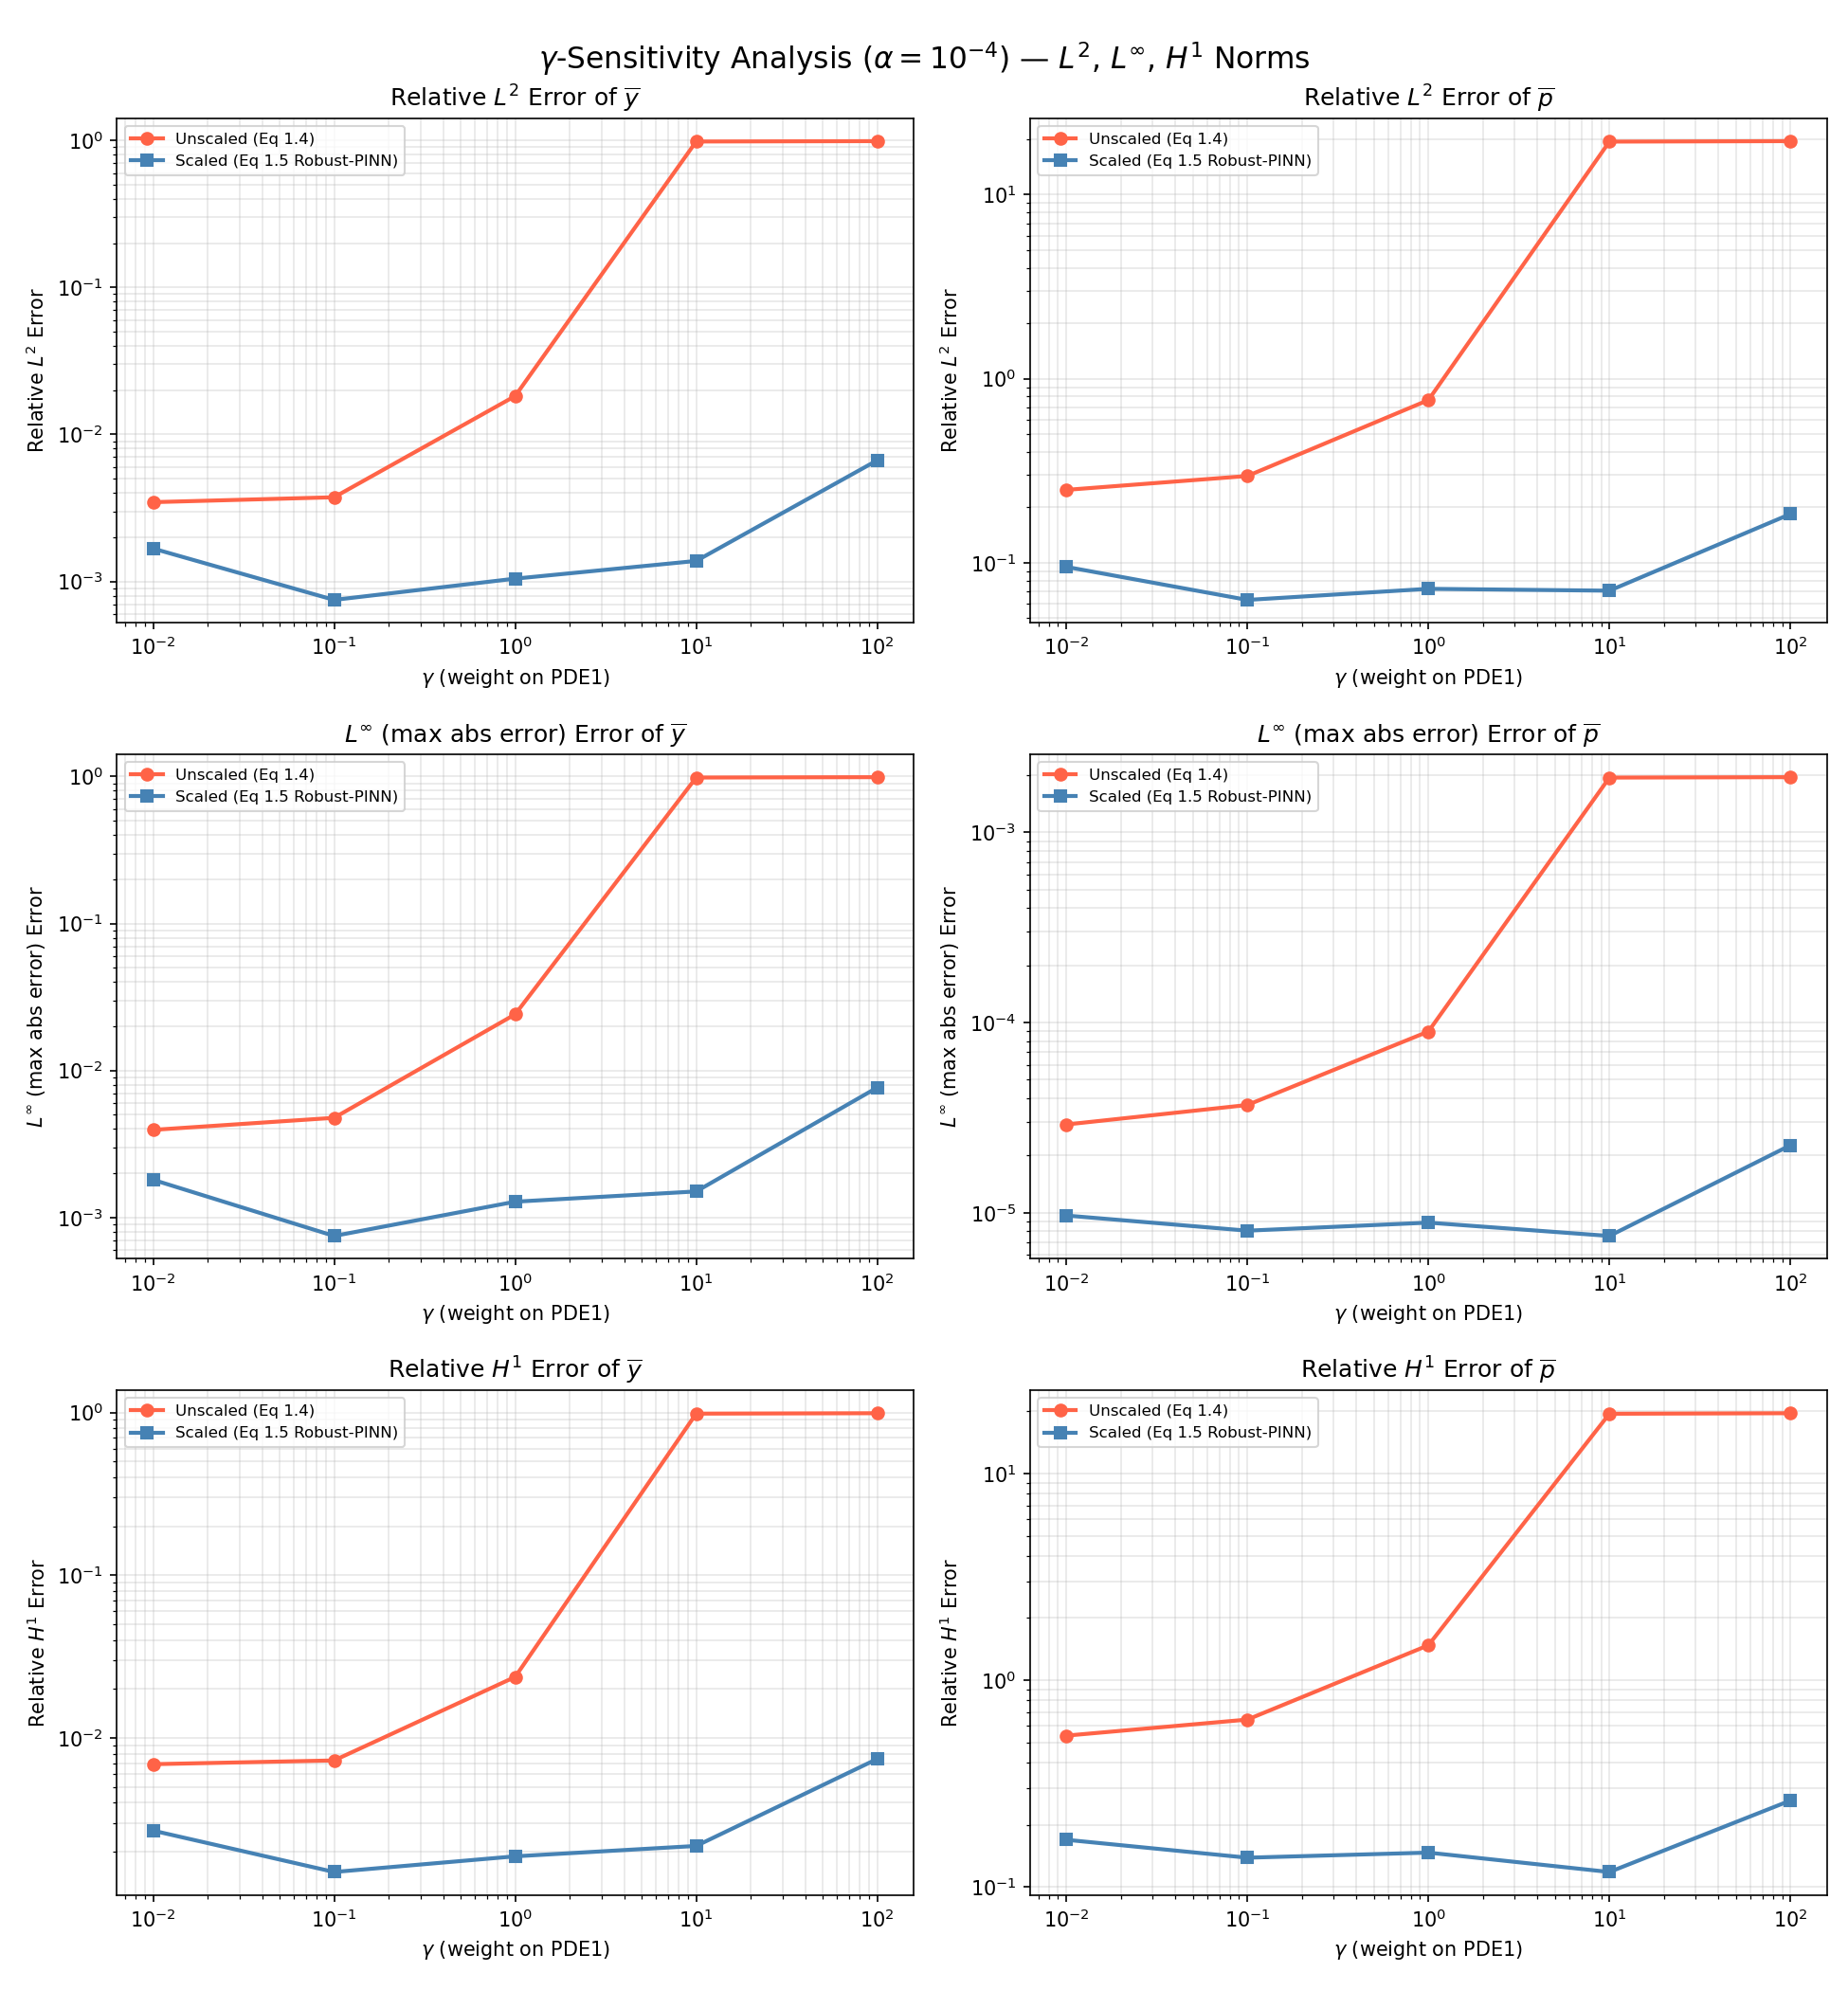
\includegraphics[width=\linewidth]{weight_test_hardBC_duelnet/weight_sensitivity_result.png}
  \caption{$\omega$-敏感性（Hard BC + Dual Network，$\alpha=10^{-4}$）：
           $L^2$、$L^\infty$、$H^1$ 误差随 $\omega$ 的变化}
  \label{fig:omega-hard-dual}
\end{figure}


% ------------------------------------------------------------------
\subsubsection{Hard BC + Unified Network}

\begin{table}[H]
  \centering
  \caption{$\omega$-敏感性实验：Hard BC + Unified Network（$\alpha=10^{-4}$）}
  \label{tab:omega-hard-unified}
  \small
  \begin{tabular}{cc rrrr}
    \toprule
    $\omega$ & 系统 & $L^2_y$ & $L^2_p$ & $H^1_y$ & $H^1_p$ \\
    \midrule
    \multirow{2}{*}{$0.01$}
      & Unscaled & $9.35\times10^{-1}$ & $1.85\times10^{+1}$
                 & $9.35\times10^{-1}$ & $1.84\times10^{+1}$ \\
      & Scaled   & $2.29\times10^{-3}$ & $4.51\times10^{-2}$
                 & $2.32\times10^{-3}$ & $4.55\times10^{-2}$ \\
    \midrule
    \multirow{2}{*}{$0.1$}
      & Unscaled & $9.35\times10^{-1}$ & $1.85\times10^{+1}$
                 & $9.35\times10^{-1}$ & $1.84\times10^{+1}$ \\
      & Scaled   & $1.70\times10^{-3}$ & $3.38\times10^{-2}$
                 & $1.71\times10^{-3}$ & $3.42\times10^{-2}$ \\
    \midrule
    \multirow{2}{*}{$1$}
      & Unscaled & $9.33\times10^{-1}$ & $1.84\times10^{+1}$
                 & $9.33\times10^{-1}$ & $1.84\times10^{+1}$ \\
      & Scaled   & $6.85\times10^{-4}$ & $1.37\times10^{-2}$
                 & $6.95\times10^{-4}$ & $1.43\times10^{-2}$ \\
    \midrule
    \multirow{2}{*}{$10$}
      & Unscaled & $9.98\times10^{-1}$ & $1.97\times10^{+1}$
                 & $9.98\times10^{-1}$ & $1.97\times10^{+1}$ \\
      & Scaled   & $1.90\times10^{-4}$ & $4.57\times10^{-3}$
                 & $2.11\times10^{-4}$ & $6.48\times10^{-3}$ \\
    \midrule
    \multirow{2}{*}{$100$}
      & Unscaled & $1.13\times10^{-2}$ & $4.63\times10^{-1}$
                 & $1.48\times10^{-2}$ & $8.47\times10^{-1}$ \\
      & Scaled   & $2.84\times10^{-4}$ & $1.44\times10^{-2}$
                 & $4.47\times10^{-4}$ & $2.37\times10^{-2}$ \\
    \bottomrule
  \end{tabular}
\end{table}

Unified Network 下 Unscaled 系统在绝大多数 $\omega$ 值上均失效
（$L^2_y \approx 0.93$--$0.998$），仅在 $\omega = 100$ 时意外地部分恢复
（$L^2_y = 0.011$），说明其可用权重窗口极为狭窄且不可预测。
相比之下，Scaled 系统全程保持 $L^2_y \sim 10^{-4}$--$10^{-3}$，
且在 $\omega = 10$ 时达到最优（$L^2_y = 1.90\times10^{-4}$），
如图~\ref{fig:omega-hard-unified} 所示。

\begin{figure}[H]
  \centering
  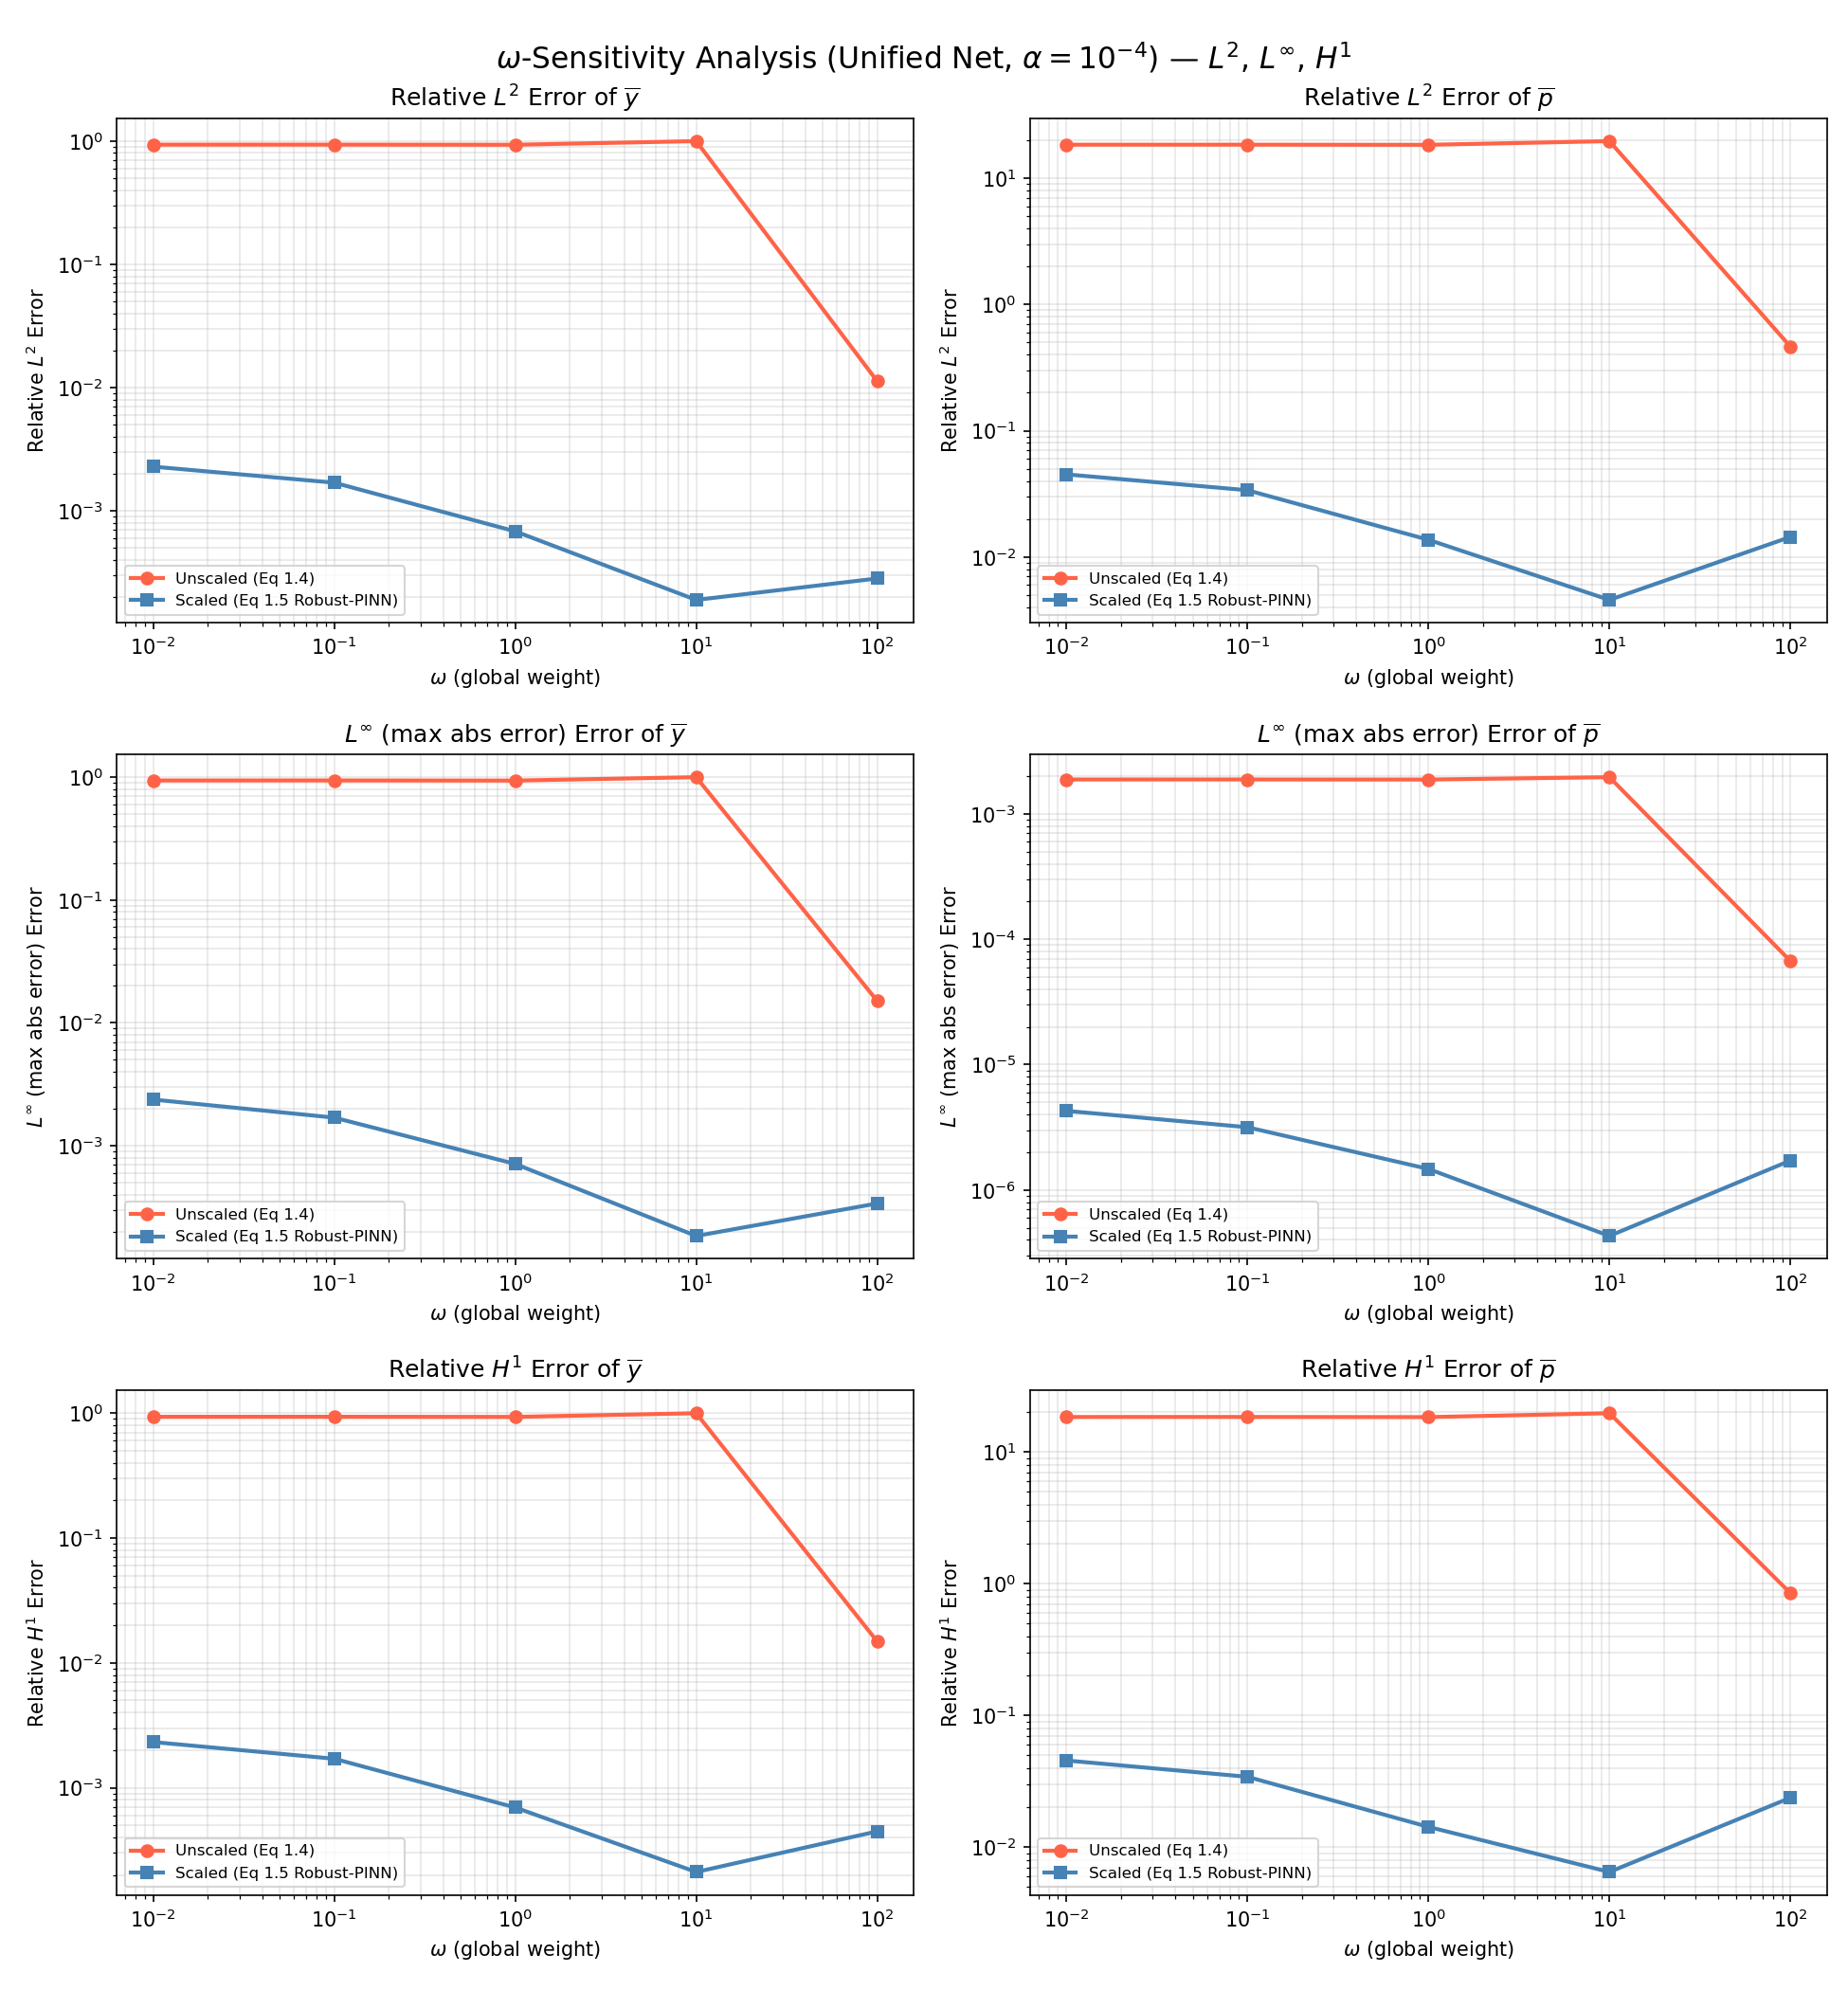
\includegraphics[width=\linewidth]{weight_test_hardBC_unified/weight_sensitivity_unified.png}
  \caption{$\omega$-敏感性（Hard BC + Unified Network，$\alpha=10^{-4}$）：
           $L^2$、$L^\infty$、$H^1$ 误差随 $\omega$ 的变化}
  \label{fig:omega-hard-unified}
\end{figure}


% ------------------------------------------------------------------
\subsubsection{Soft BC + Unified Network}

\begin{table}[H]
  \centering
  \caption{$\omega$-敏感性实验：Soft BC + Unified Network（$\alpha=10^{-4}$）}
  \label{tab:omega-soft-unified}
  \small
  \begin{tabular}{cc rrrr}
    \toprule
    $\omega$ & 系统 & $L^2_y$ & $L^2_p$ & $H^1_y$ & $H^1_p$ \\
    \midrule
    \multirow{2}{*}{$0.01$}
      & Unscaled & $9.93\times10^{-1}$ & $1.95\times10^{+1}$
                 & $9.99\times10^{-1}$ & $1.95\times10^{+1}$ \\
      & Scaled   & $4.21\times10^{-2}$ & $8.37\times10^{-1}$
                 & $4.25\times10^{-2}$ & $8.37\times10^{-1}$ \\
    \midrule
    \multirow{2}{*}{$0.1$}
      & Unscaled & $9.38\times10^{-1}$ & $1.94\times10^{+1}$
                 & $9.96\times10^{-1}$ & $1.94\times10^{+1}$ \\
      & Scaled   & $3.72\times10^{-2}$ & $7.83\times10^{-1}$
                 & $3.99\times10^{-2}$ & $7.83\times10^{-1}$ \\
    \midrule
    \multirow{2}{*}{$1$}
      & Unscaled & $7.05\times10^{-1}$ & $1.94\times10^{+1}$
                 & $9.87\times10^{-1}$ & $1.95\times10^{+1}$ \\
      & Scaled   & $1.56\times10^{-2}$ & $4.38\times10^{-1}$
                 & $2.41\times10^{-2}$ & $4.39\times10^{-1}$ \\
    \midrule
    \multirow{2}{*}{$10$}
      & Unscaled & $5.96\times10^{-1}$ & $1.93\times10^{+1}$
                 & $9.83\times10^{-1}$ & $1.91\times10^{+1}$ \\
      & Scaled   & $2.10\times10^{-2}$ & $7.37\times10^{-1}$
                 & $4.25\times10^{-2}$ & $7.45\times10^{-1}$ \\
    \midrule
    \multirow{2}{*}{$100$}
      & Unscaled & $6.12\times10^{-1}$ & $1.98\times10^{+1}$
                 & $9.94\times10^{-1}$ & $2.05\times10^{+1}$ \\
      & Scaled   & $1.15\times10^{-2}$ & $4.00\times10^{-1}$
                 & $2.26\times10^{-2}$ & $4.56\times10^{-1}$ \\
    \bottomrule
  \end{tabular}
\end{table}

软边界下 Unscaled 的 $L^2_y$ 在 $0.59$--$0.99$ 之间剧烈波动，
$L^2_p$ 始终 $\approx 19$（完全未学到 $\bar{p}$）；
Scaled 的 $L^2_y$ 稳定在 $0.01$--$0.04$，
在所有 $\omega$ 下均保持 $1$--$2$ 个量级的显著优势
（图~\ref{fig:omega-soft-unified}）。

\begin{figure}[H]
  \centering
  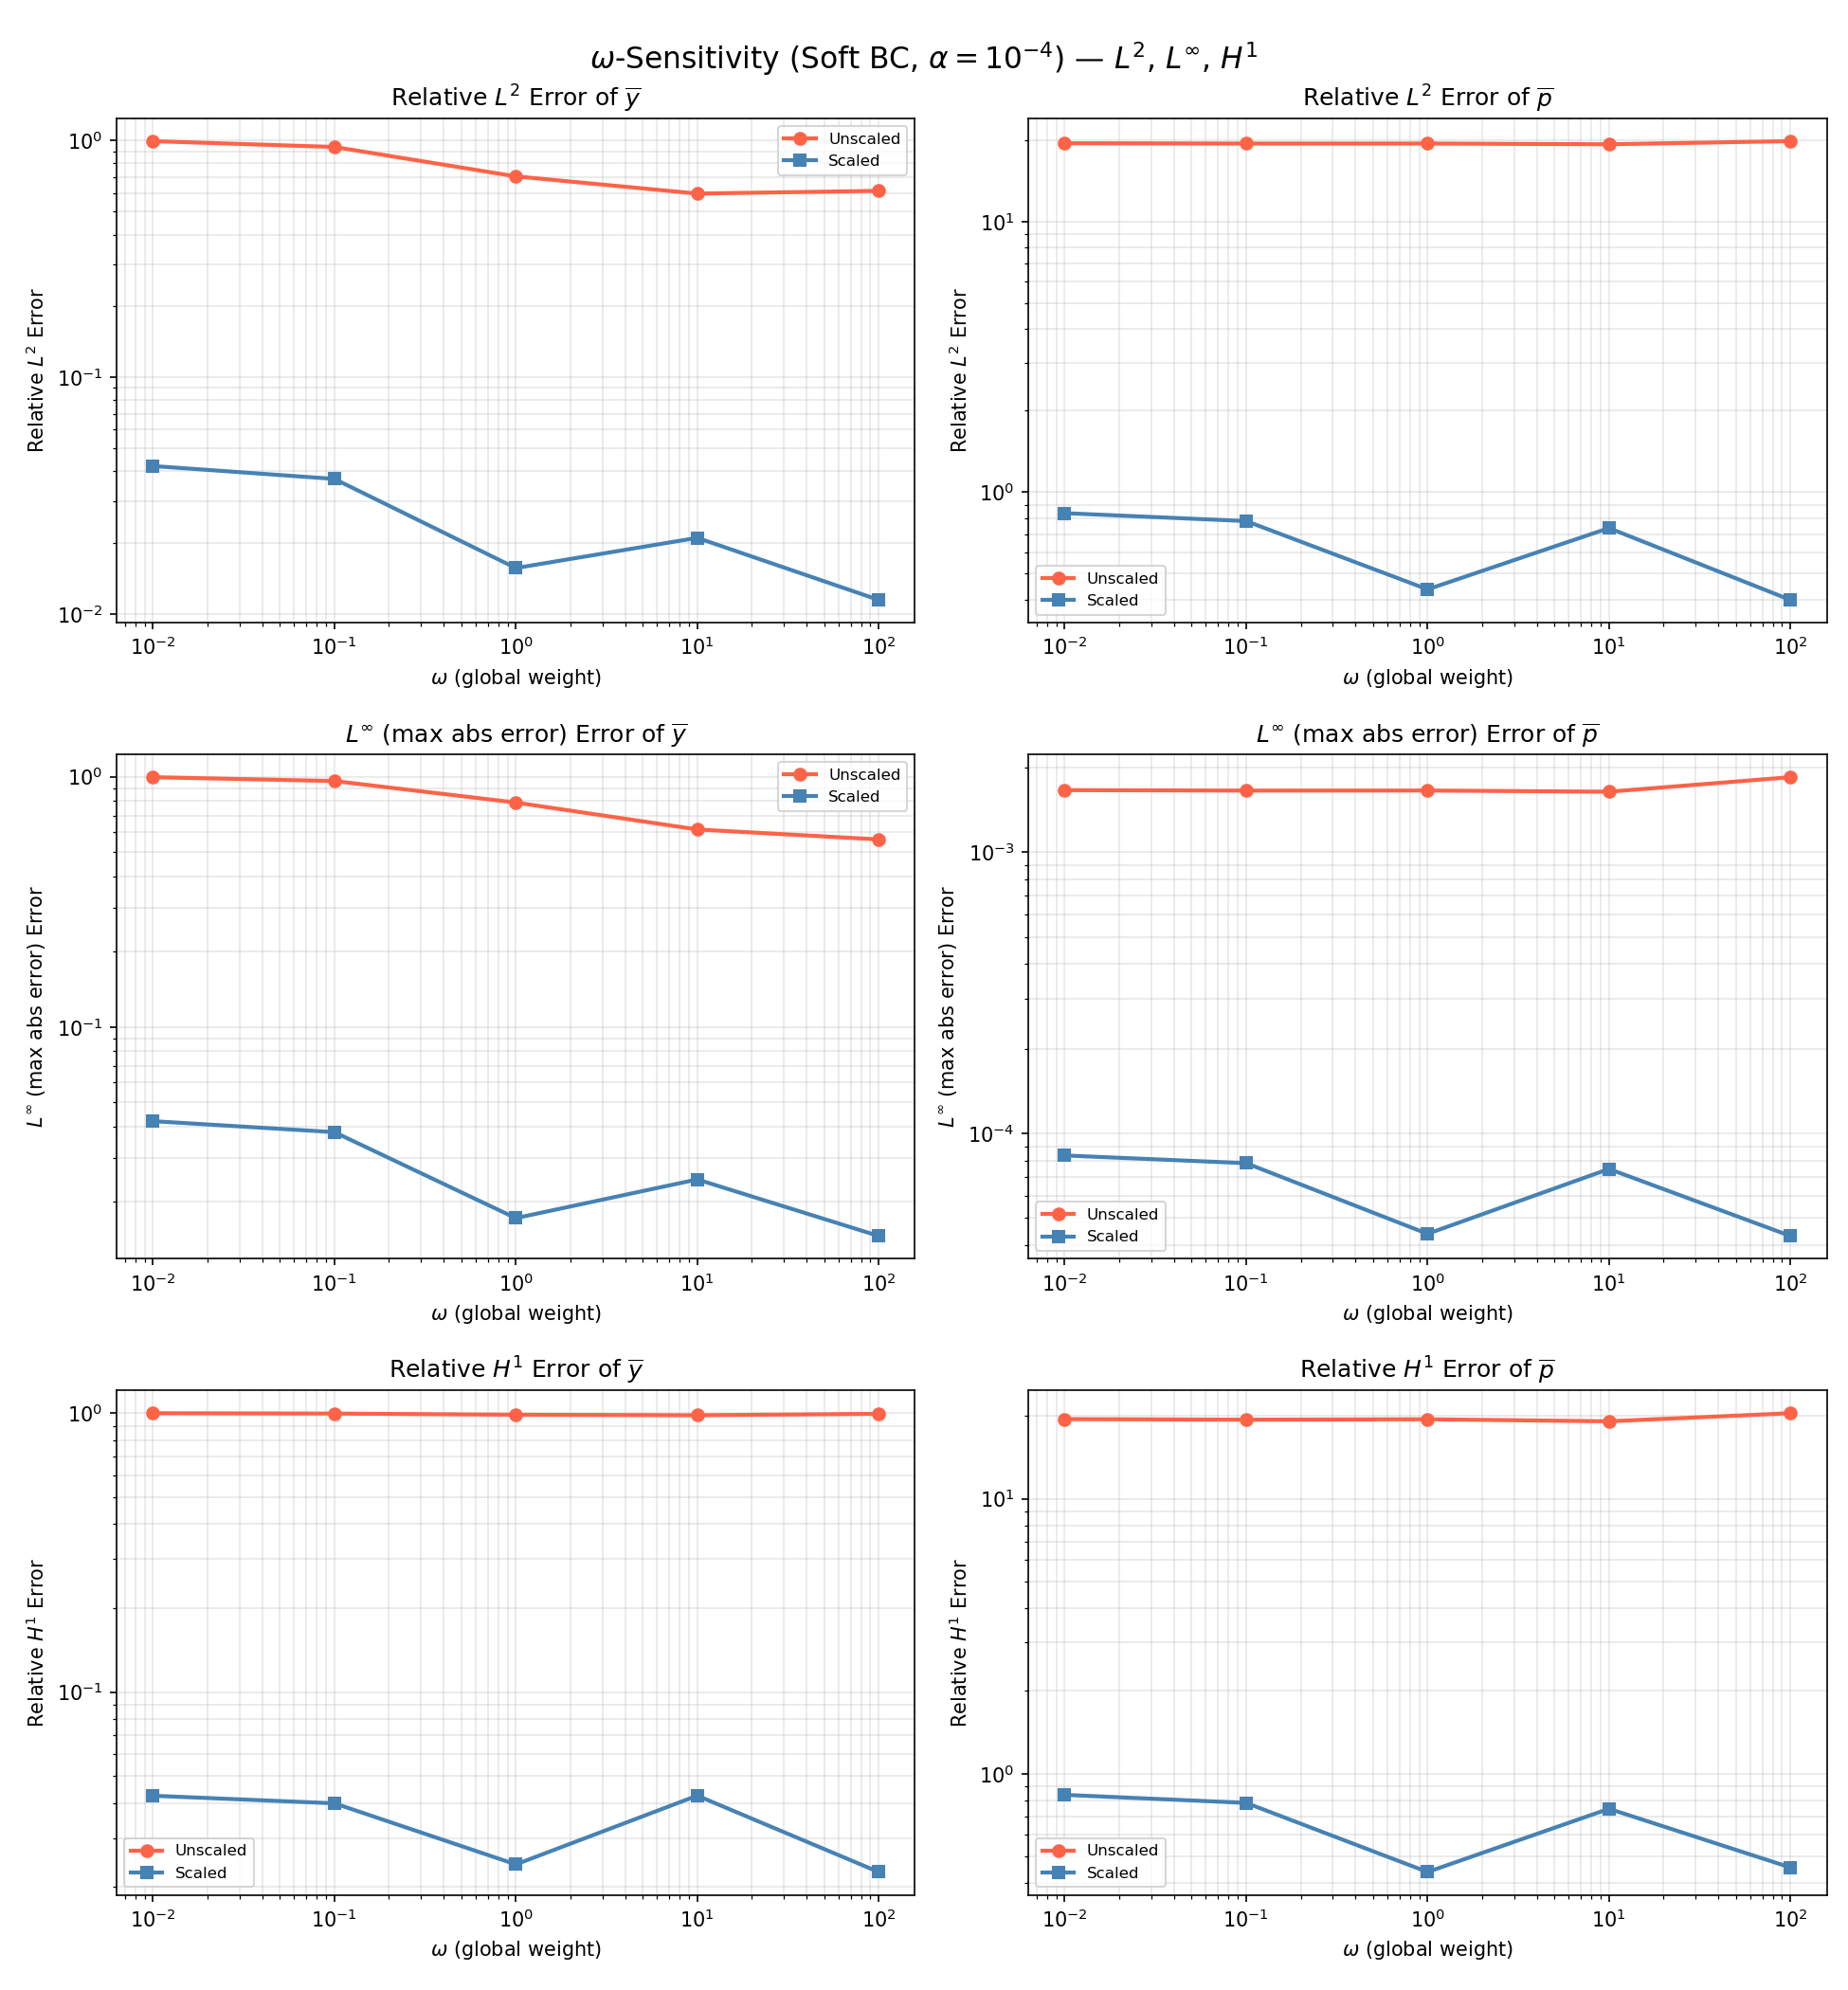
\includegraphics[width=\linewidth]{weight_test_softBC_unified/weight_sensitivity_soft_bc.png}
  \caption{$\omega$-敏感性（Soft BC + Unified Network，$\alpha=10^{-4}$）：
           $L^2$、$L^\infty$、$H^1$ 误差随 $\omega$ 的变化}
  \label{fig:omega-soft-unified}
\end{figure}


% ------------------------------------------------------------------
\subsubsection{$\omega$-敏感性实验小结}

三组实验一致表明：
\begin{enumerate}
  \item Unscaled 系统对 $\omega$ 极度敏感：在 Hard BC + Dual Network 下仅
        $\omega \leq 1$ 可用，在 Unified Network 下几乎全军覆没；
  \item Scaled 系统在 $\omega$ 跨越 4 个量级（$0.01$--$100$）的范围内保持误差稳定，
        符合定理~\ref{thm:stiffness} 的刚度比压缩预测；
  \item Hard BC 下 Scaled 的误差波动范围仅为 $10^{-4}$--$10^{-3}$（不足 1 个量级），
        Soft BC 下约为 $10^{-2}$--$10^{-1}$（约 1 个量级），
        均远优于 Unscaled 的多个量级跳变。
\end{enumerate}


% ==================================================================
\subsection{综合分析}
\label{subsec:synthesis}

\paragraph{Hard BC vs.\ Soft BC。}
Hard BC 通过距离函数 Ansatz 精确满足边界条件，使网络仅需优化内部 PDE 残差，
是 Scaling 效果最理想的场景（$L^2 \sim 10^{-4}$）。
Soft BC 引入了边界与内部残差的竞争，绝对精度降低约 $1$--$2$ 个量级
（$L^2 \sim 10^{-2}$），但 Scaling 的相对优势依然显著。
在实际应用中，复杂几何往往使 Hard BC 不可用，
而 Soft BC + Scaling + 边界归一化的组合仍能保证数量级的改进。

\paragraph{Unified Network vs.\ Dual Network。}
Unified 架构通过参数共享天然引入 $y$ 与 $p$ 的隐式耦合，
在所有实验配置下均表现优于 Dual Network。
尤其在 Soft BC 下，Dual Network 的 $\bar{p}$ 几乎完全丧失
（$L^2_p \approx 1.0$），而 Unified Network 的 $L^2_p$ 可降至 $\sim\!0.2$。

\paragraph{残差归一化的关键作用。}
Scaled 系统的两个 PDE 残差 $R_1$、$R_2$ 仍分别携带 $\alpha^{3/4}$、$\alpha^{1/4}$
的量级因子。逐残差归一化（除以各自特征尺度）进一步消除残余的量级不平衡。
在 Soft BC 下，边界项的归一化同样关键：
未做归一化时精度明显退化
（如图~\ref{fig:alpha-soft-unified-unnorm} 所示）。

\begin{figure}[H]
  \centering
  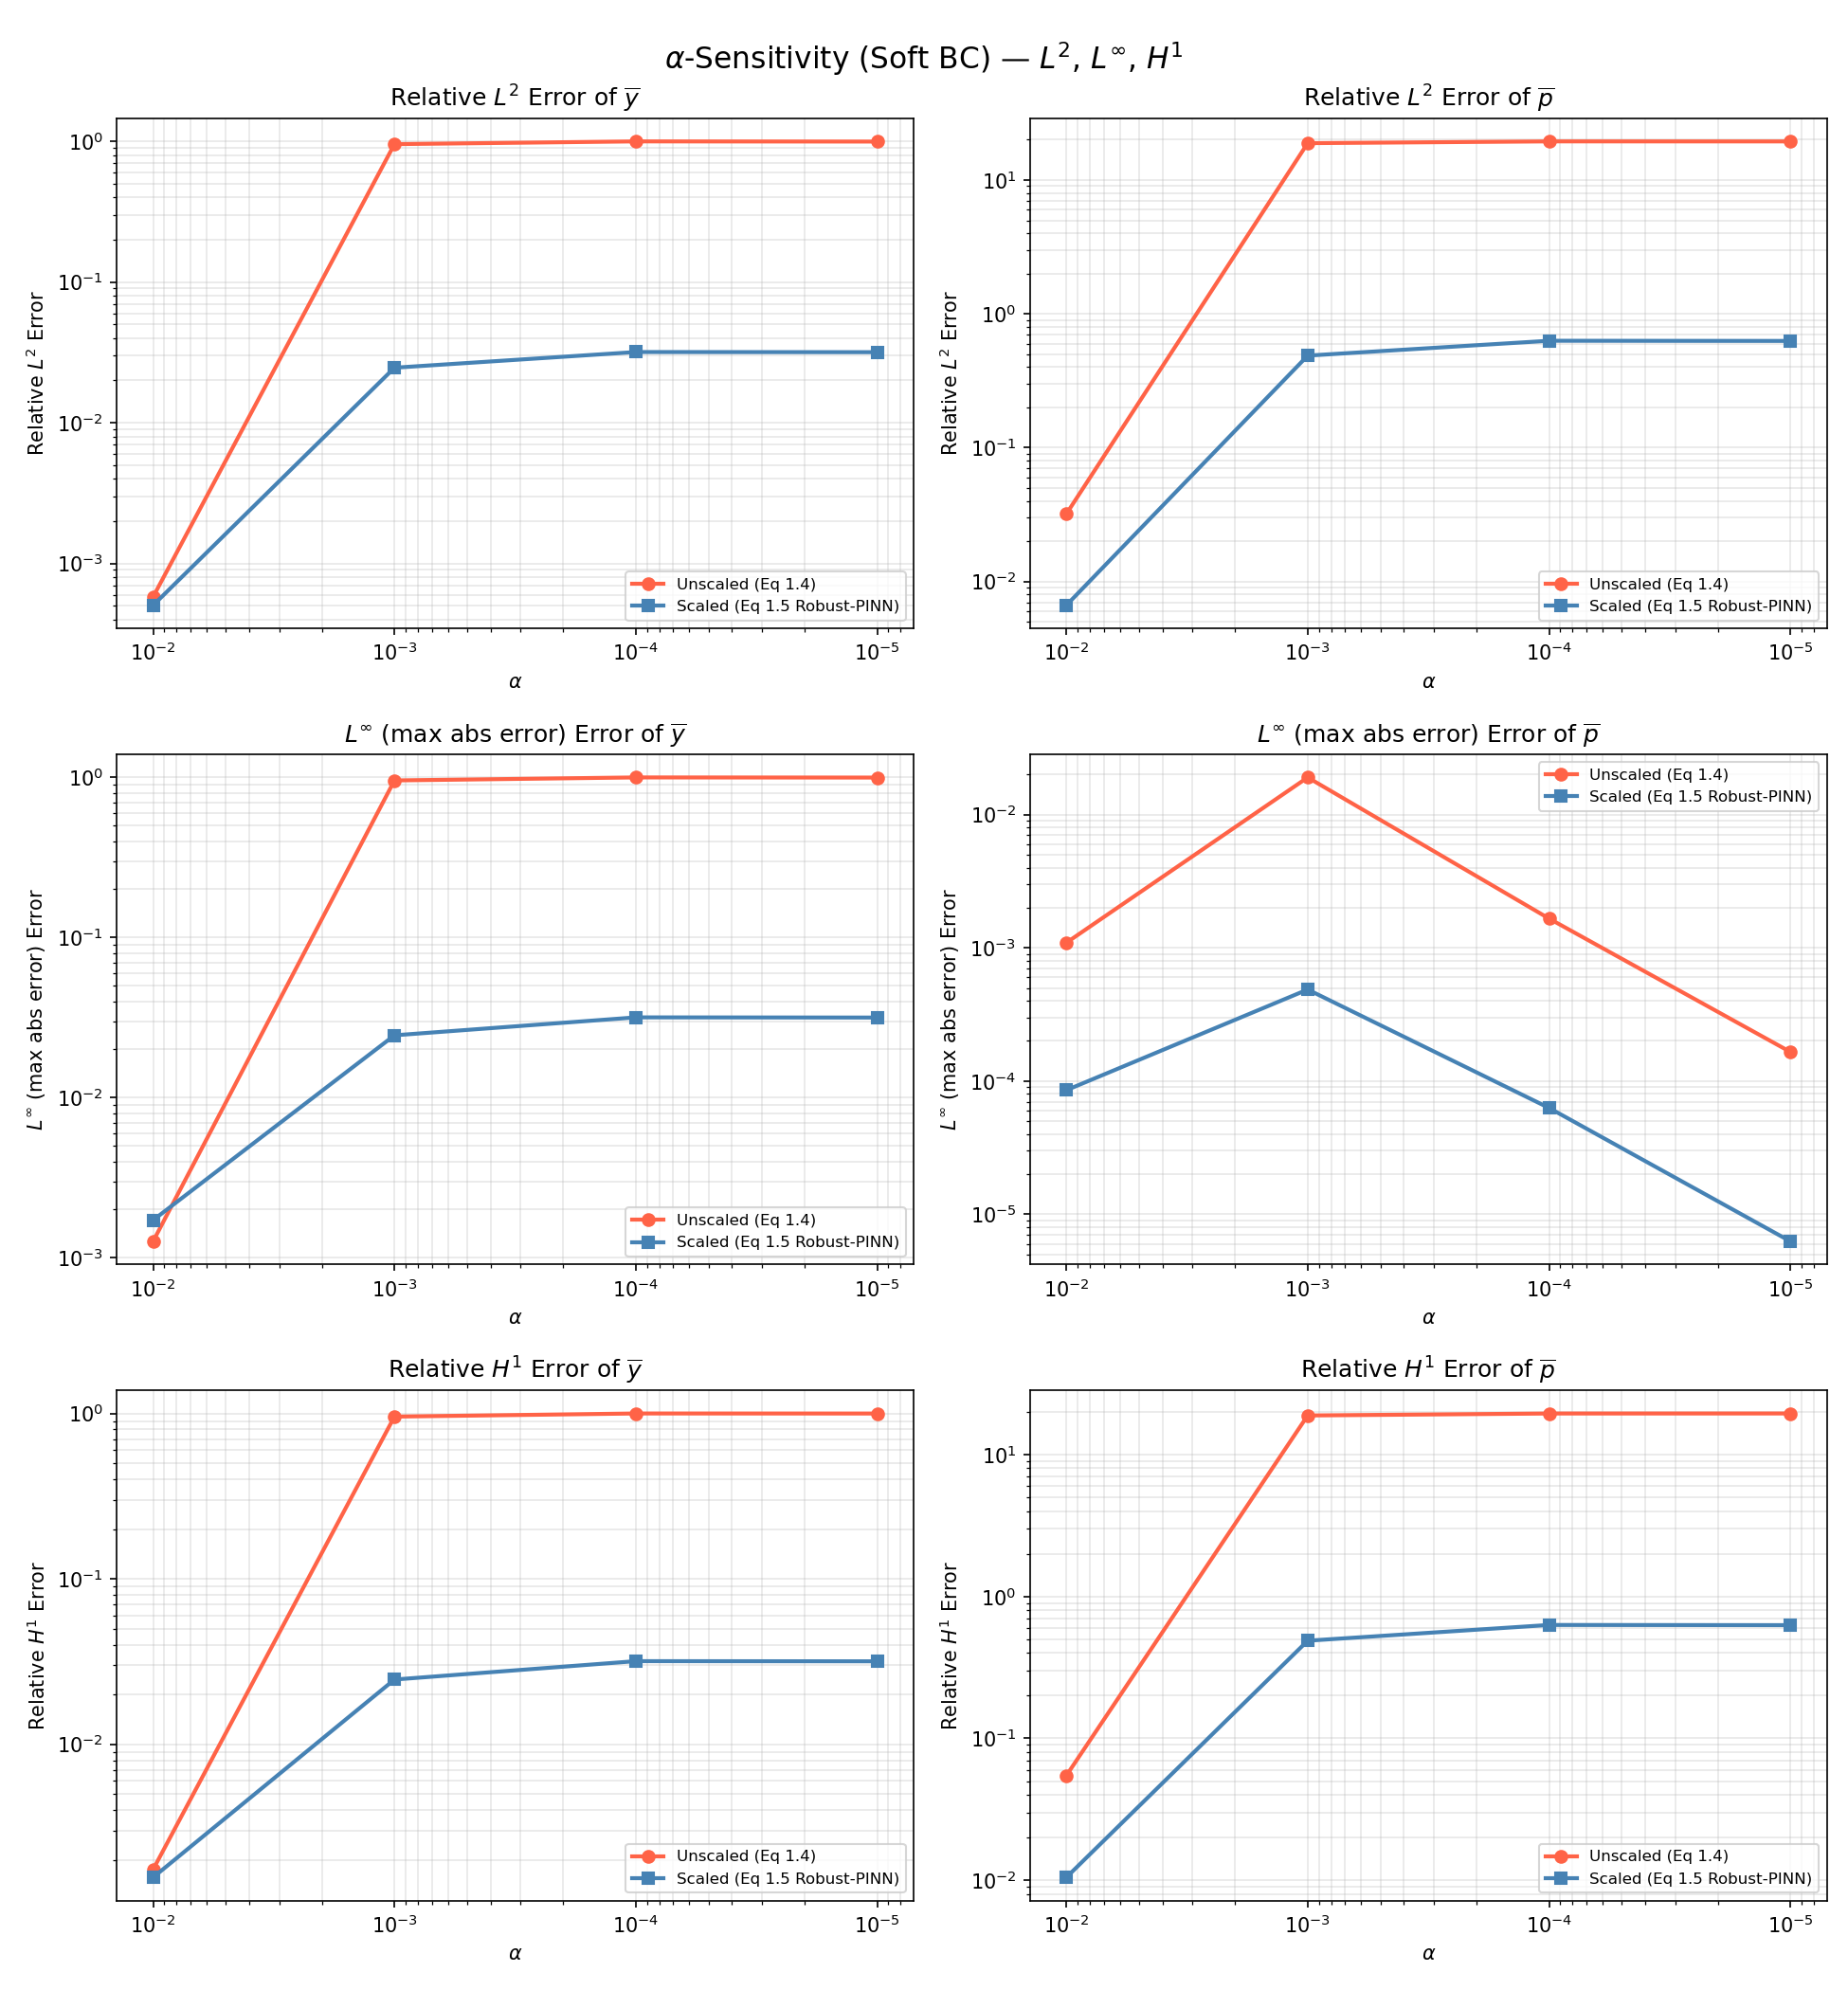
\includegraphics[width=\linewidth]{alpha_test_softBC_unified/unified_sensitivity_soft_bc_result.png}
  \caption{Soft BC + Unified Network 中残差归一化对 Scaled 系统精度的影响}
  \label{fig:alpha-soft-unified-unnorm}
\end{figure}

\paragraph{核心结论。}
六组实验从 $\alpha$-敏感性和 $\omega$-敏感性两个维度，
在 Unified / Dual Network $\times$ Hard / Soft BC 的四种配置下，
系统性地验证了以下结论：
\begin{enumerate}
  \item (1.5) 式 Scaling 变换有效地将参数依赖问题转化为近参数无关问题，
        数值结果与梯度渐近分析（定理~\ref{thm:gradient-divergence}）
        及刚度比分析（定理~\ref{thm:stiffness}）的理论预测高度吻合；
  \item Scaling 同时降低了对 $\alpha$ 和 $\omega$ 的敏感性，
        使得实际应用中无需精细调参即可获得稳定的求解精度；
  \item 该策略对网络架构和边界处理方式具有普适性，
        是构建 Robust-PINN 求解最优控制问题的核心保障。
\end{enumerate}


% ==================================================================
\section{Part 1 解法说明}
\label{sec:part1}

\begin{figure}[H]
  \centering
  \includegraphics[width=0.85\linewidth]{part1_loss_comparison_20260301_091035.png}
  \caption{Part 1 各损失分量演化曲线}
  \label{fig:loss}
\end{figure}

\begin{figure}[H]
  \centering
  \includegraphics[width=\linewidth]{part1_solution_20260301_091035.png}
  \caption{Part 1 数值解与精确解对比}
  \label{fig:sol}
\end{figure}

\subsection{Fourier Feature Embedding 的引入}

在基本完成方法后，为排除过拟合，对 $f$ 进行了调整以测试模型的泛化能力。
在提高频率的过程中发现，模型对高频方程的处理能力不足，
于是加入了随机 Fourier 特征处理，使得模型在频率提高时依旧有良好表现。

\subsection{优化器 L-BFGS 的引入}

在加入 L-BFGS 之前，模型的误差量级虽然下降了，但结果一直处于震荡状态（图~\ref{fig:loss-no-lbfgs}）。

\begin{figure}[H]
  \centering
  \includegraphics[width=0.8\linewidth]{part1_loss_comparison_20260301_085239.png}
  \caption{未使用 L-BFGS 时的损失曲线——收敛震荡明显}
  \label{fig:loss-no-lbfgs}
\end{figure}

在 PINN 经典论文~\cite{pinn_paper}及其参考文献~\cite{liu1989lbfgs}中，均选用了与 Adam
等一阶优化器不同的、更适合 PINN 损失函数的优化器——L-BFGS。其核心特性如下：

\begin{enumerate}[label=(\roman*)]
  \item \textbf{利用曲率信息（拟牛顿法）：}
    L-BFGS 通过保存历史梯度的变化，近似构造 Hessian 矩阵。
    当 $\mathrm{MSE}_u$ 和 $\mathrm{MSE}_f$ 的梯度相互拉扯导致普通优化器原地打转时，
    L-BFGS 能通过曲率信息"看穿"震荡，计算出使总损失同时下降的最优牛顿方向。

  \item \textbf{全批量评估（Full-batch）：}
    L-BFGS 是全批量算法——所有边界点和内部配点在每次迭代中完全固定并一次性输入。
    只有这样，损失函数的"地形"才是静止的，L-BFGS 的线搜索才能精准找到谷底。
\end{enumerate}

L-BFGS 的高收敛精度，使得物理残差正则化项被逼近机器精度，
从而在无网格划分（PINN 特性）的情况下，精准捕捉方程内部复杂的动态行为。


% ==================================================================
\section{数值实验}
\label{sec:experiments}

实验思路：为验证 Scaling 处理对敏感度降低的有效性，采用两种策略进行验证：
\begin{itemize}
  \item \textbf{策略一}：固定损失函数权重，验证误差对 $\alpha$ 的变化不敏感。
  \item \textbf{策略二}：将 $\alpha$ 固定在较为病态的数值，验证误差对损失函数权重变化不敏感。
\end{itemize}

% ------------------------------------------------------------------
\subsection{策略一：$\alpha$ 敏感性测试}
\label{subsec:alpha-sensitivity}

\begin{table}[H]
  \centering
  \caption{$\alpha$ 敏感性实验结果}
  \label{tab:alpha-sensitivity}
  \begin{tabular}{ccccc}
    \toprule
    $\alpha$ & System   & $\mathrm{Err}_y$ & $\mathrm{Err}_p$ & Time (s) \\
    \midrule
    $10^{-2}$ & Unscaled & $6.85\times10^{-5}$  & $4.30\times10^{-3}$  & 142.6 \\
    $10^{-2}$ & Scaled   & $5.90\times10^{-5}$  & $3.24\times10^{-3}$  & 157.4 \\
    \midrule
    $10^{-3}$ & Unscaled & $3.92\times10^{-4}$  & $2.64\times10^{-2}$  & 140.6 \\
    $10^{-3}$ & Scaled   & $8.80\times10^{-4}$  & $4.80\times10^{-2}$  & 164.4 \\
    \midrule
    $10^{-4}$ & Unscaled & $1.82\times10^{-2}$  & $7.65\times10^{-1}$  & 112.8 \\
    $10^{-4}$ & Scaled   & $1.04\times10^{-3}$  & $7.21\times10^{-2}$  & 139.2 \\
    \midrule
    $10^{-5}$ & Unscaled & $9.71\times10^{-1}$  & $1.92\times10^{+1}$  & 109.7 \\
    $10^{-5}$ & Scaled   & $9.91\times10^{-4}$  & $6.68\times10^{-2}$  & 140.7 \\
    \bottomrule
  \end{tabular}
\end{table}

\begin{figure}[H]
  \centering
  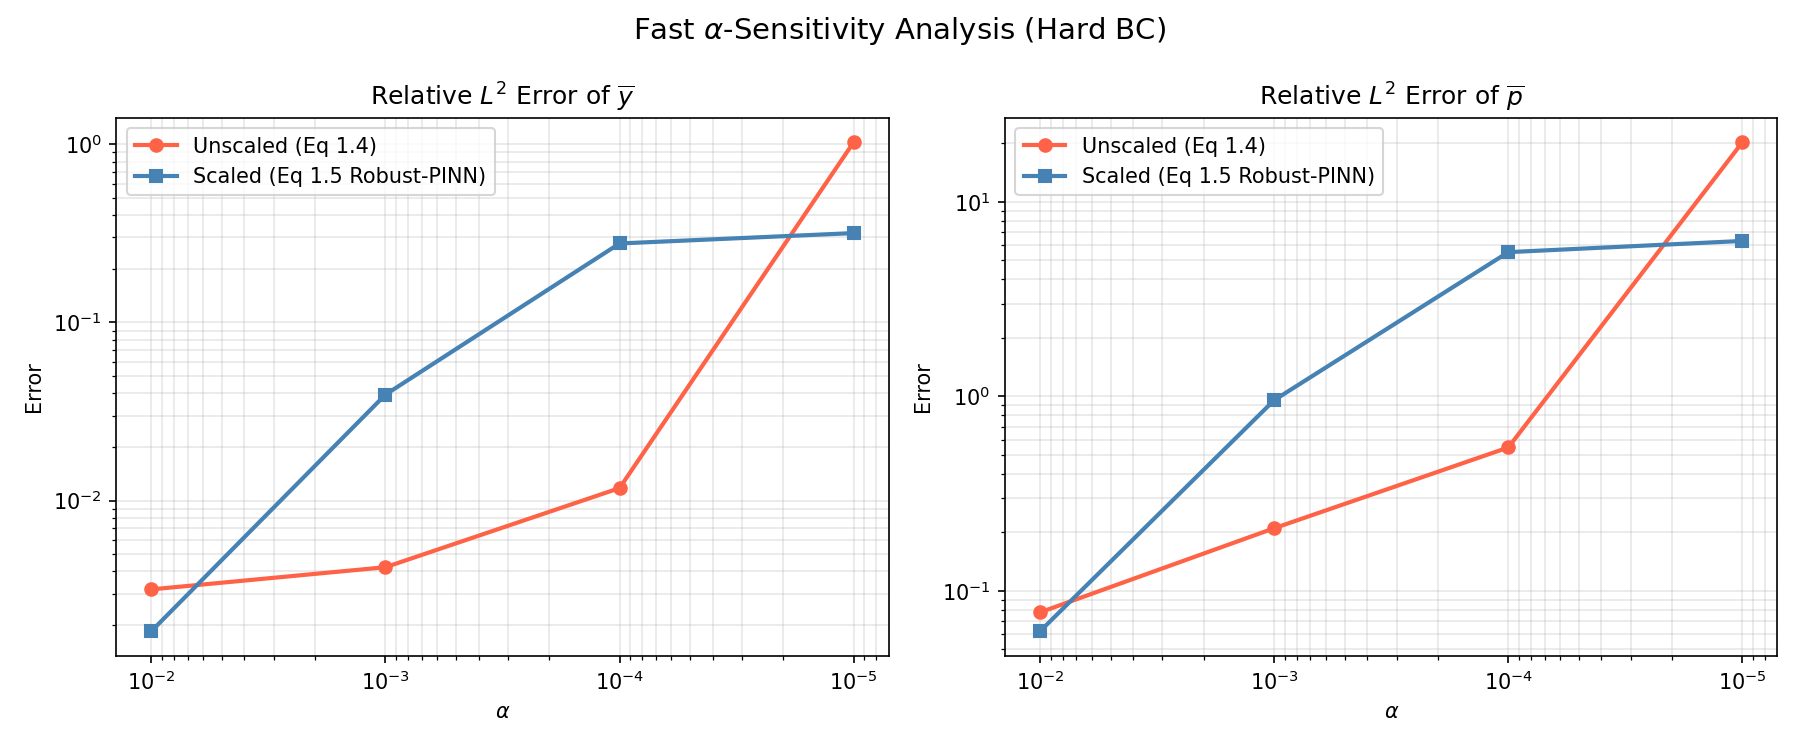
\includegraphics[width=\linewidth]{fast_sensitivity_result.png}
  \caption{$\alpha$ 敏感性实验：相对 $L^2$ 误差随 $\alpha$ 的变化}
  \label{fig:alpha-sensitivity}
\end{figure}

% ------------------------------------------------------------------
\subsection{策略二：损失权重敏感性测试}
\label{subsec:weight-sensitivity}

\begin{table}[H]
  \centering
  \caption{损失权重 $\gamma$ 敏感性实验结果（$\alpha=10^{-4}$）}
  \label{tab:weight-sensitivity}
  \begin{tabular}{ccccc}
    \toprule
    $\gamma$ & System & $\mathrm{Err}_y$ & $\mathrm{Err}_p$ & Time (s) \\
    \midrule
    $0.01$  & Unscaled & $3.46\times10^{-3}$ & $2.49\times10^{-1}$ & 105.7 \\
    $0.01$  & Scaled   & $1.67\times10^{-3}$ & $9.49\times10^{-2}$ & 109.9 \\
    \midrule
    $0.10$  & Unscaled & $3.74\times10^{-3}$ & $2.96\times10^{-1}$ & 100.3 \\
    $0.10$  & Scaled   & $7.48\times10^{-4}$ & $6.28\times10^{-2}$ & 125.9 \\
    \midrule
    $1.00$  & Unscaled & $1.82\times10^{-2}$ & $7.65\times10^{-1}$ & 114.3 \\
    $1.00$  & Scaled   & $1.04\times10^{-3}$ & $7.21\times10^{-2}$ & 135.9 \\
    \midrule
    $10.00$ & Unscaled & $9.84\times10^{-1}$ & $1.94\times10^{+1}$ & 108.6 \\
    $10.00$ & Scaled   & $1.38\times10^{-3}$ & $7.04\times10^{-2}$ & 215.7 \\
    \midrule
    $100.00$ & Unscaled & $9.90\times10^{-1}$ & $1.95\times10^{+1}$ & 111.8 \\
    $100.00$ & Scaled   & $6.67\times10^{-3}$ & $1.84\times10^{-1}$ & 150.7 \\
    \bottomrule
  \end{tabular}
\end{table}

\begin{figure}[H]
  \centering
  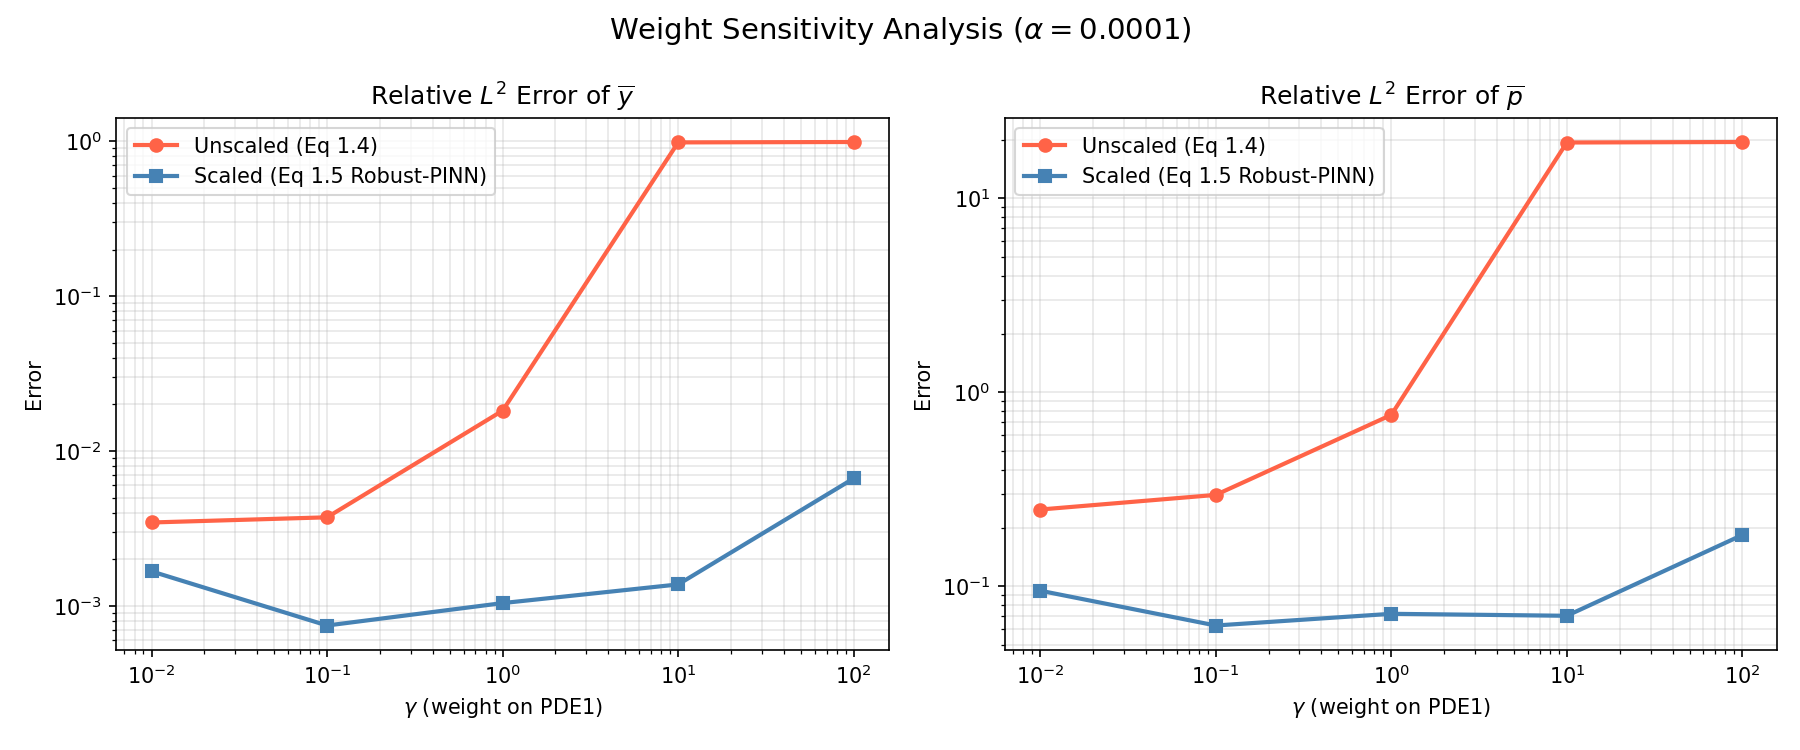
\includegraphics[width=\linewidth]{weight_sensitivity_result.png}
  \caption{损失权重 $\gamma$ 敏感性实验：相对 $L^2$ 误差随 $\gamma$ 的变化}
  \label{fig:weight-sensitivity}
\end{figure}


% ==================================================================
\subsection{基础数学定义}
\label{subsec:math-defs}

设神经网络的参数为 $\theta = [\theta_y,\;\theta_p]^\mathsf{T}$。
在 PINNs 中，将状态变量和伴随状态变量参数化为
$\overline{y}_\theta,\;\overline{p}_\theta$（未缩放）和 $y_\theta,\;p_\theta$（缩放）。

\paragraph{未缩放系统的残差与损失.}
根据一阶最优性系统，定义：
\begin{align}
  R_{1,\mathrm{un}}(\theta) &= -\Delta\overline{y}_\theta - f - u_d + \alpha^{-1}\overline{p}_\theta, \label{eq:R1-un}\\
  R_{2,\mathrm{un}}(\theta) &= -\Delta\overline{p}_\theta - \overline{y}_\theta + y_d. \label{eq:R2-un}
\end{align}
未缩放的损失函数为：
\begin{equation}
  \mathcal{L}_{\mathrm{un}}(\theta)
  = w_1\|R_{1,\mathrm{un}}(\theta)\|^2 + w_2\|R_{2,\mathrm{un}}(\theta)\|^2.
  \label{eq:loss-un}
\end{equation}

\paragraph{缩放系统的残差与损失.}
\begin{align}
  R_{1,\mathrm{sc}}(\theta) &= -\alpha^{1/2}\Delta y_\theta + p_\theta - \alpha^{3/4}(f + u_d), \label{eq:R1-sc}\\
  R_{2,\mathrm{sc}}(\theta) &= -\alpha^{1/2}\Delta p_\theta - y_\theta + \alpha^{1/4}y_d. \label{eq:R2-sc}
\end{align}
缩放后的损失函数为：
\begin{equation}
  \mathcal{L}_{\mathrm{sc}}(\theta)
  = w_1\|R_{1,\mathrm{sc}}(\theta)\|^2 + w_2\|R_{2,\mathrm{sc}}(\theta)\|^2.
  \label{eq:loss-sc}
\end{equation}


% ------------------------------------------------------------------
\subsection{策略一证明：$\alpha\to 0$ 时的梯度渐近稳定性}
\label{subsec:proof-alpha}

\begin{theorem}[梯度发散与有界性]
\label{thm:gradient-divergence}
当权重 $w_1, w_2$ 固定，且 $\alpha\to 0$ 时：
\begin{enumerate}[label=(\alph*)]
  \item 未缩放损失函数关于 $\theta_p$ 的梯度范数趋于无穷：
    $\displaystyle\lim_{\alpha\to 0}\|\nabla_{\theta_p}\mathcal{L}_{\mathrm{un}}\| = \infty$；
  \item 缩放后损失函数的梯度范数严格有界：
    $\displaystyle\lim_{\alpha\to 0}\|\nabla_\theta\mathcal{L}_{\mathrm{sc}}\| < \infty$。
\end{enumerate}
\end{theorem}

\begin{proof}
\textbf{(a) 未缩放系统.}\;
考察损失函数对 $\theta_p$ 的梯度：
\begin{equation}
  \nabla_{\theta_p}\mathcal{L}_{\mathrm{un}}
  = 2w_1\langle R_{1,\mathrm{un}},\;\nabla_{\theta_p}R_{1,\mathrm{un}}\rangle
  + 2w_2\langle R_{2,\mathrm{un}},\;\nabla_{\theta_p}R_{2,\mathrm{un}}\rangle.
  \label{eq:grad-un}
\end{equation}
其中 $\nabla_{\theta_p}R_{1,\mathrm{un}} = \alpha^{-1}\nabla_{\theta_p}\overline{p}_\theta$。
代入并提取 $\alpha$ 因子：
\begin{equation}
  \nabla_{\theta_p}\mathcal{L}_{\mathrm{un}}
  = \underbrace{\alpha^{-2}\bigl[2w_1\langle\overline{p}_\theta,\;\nabla_{\theta_p}\overline{p}_\theta\rangle\bigr]}_{\text{主导项}}
  + \alpha^{-1}\bigl[2w_1\langle -\Delta\overline{y}_\theta - f - u_d,\;\nabla_{\theta_p}\overline{p}_\theta\rangle\bigr]
  + \mathcal{O}(1).
  \label{eq:grad-un-expand}
\end{equation}
当 $\alpha\to 0$ 时，主导项为 $\mathcal{O}(\alpha^{-2})$，梯度严重爆炸。

\medskip
\textbf{(b) 缩放系统.}\;
考察梯度：
\begin{equation}
  \nabla_\theta\mathcal{L}_{\mathrm{sc}}
  = 2w_1\langle R_{1,\mathrm{sc}},\;\nabla_\theta R_{1,\mathrm{sc}}\rangle
  + 2w_2\langle R_{2,\mathrm{sc}},\;\nabla_\theta R_{2,\mathrm{sc}}\rangle,
  \label{eq:grad-sc}
\end{equation}
其中
\begin{align}
  \nabla_{\theta_p}R_{1,\mathrm{sc}} &= \nabla_{\theta_p}p_\theta
    &\text{（系数为 $1$）},   \label{eq:grad-sc-R1}\\
  \nabla_{\theta_p}R_{2,\mathrm{sc}} &= -\alpha^{1/2}\nabla_{\theta_p}(\Delta p_\theta)
    &\text{（系数为 $\mathcal{O}(\alpha^{1/2})$）}. \label{eq:grad-sc-R2}
\end{align}
所有项包含的 $\alpha$ 因子均为正数次幂（$\alpha^{1/2},\;\alpha^{1/4},\;\alpha^{3/4}$）或常数 $1$。
因此 $\|\nabla_\theta\mathcal{L}_{\mathrm{sc}}\| = \mathcal{O}(1)$，不存在梯度爆炸。
\end{proof}

% ------------------------------------------------------------------
\subsection{策略二证明：固定极小 $\alpha$ 下的梯度刚性分析}
\label{subsec:proof-weight}

\begin{theorem}[梯度刚性抑制]
\label{thm:stiffness}
定义系统刚度比为
$\kappa = \|\nabla_\theta\mathcal{L}_1\| \big/ \|\nabla_\theta\mathcal{L}_2\|$。
在 $\alpha\ll 1$ 下：
\begin{enumerate}[label=(\alph*)]
  \item 未缩放系统：$\kappa_{\mathrm{un}} = \mathcal{O}(\alpha^{-2})$，对权重 $w_1,w_2$ 极度敏感；
  \item 缩放系统：$\kappa_{\mathrm{sc}}$ 被压缩至 $\mathcal{O}(\alpha^{-1/2})$ 乃至 $\mathcal{O}(1)$。
\end{enumerate}
\end{theorem}

\begin{proof}
设 $\alpha$ 为极小的固定正数（如 $10^{-4}$）。

\textbf{未缩放系统.}\;
两项损失产生的梯度范数分别为：
\begin{align}
  \|\nabla_\theta(w_1\|R_{1,\mathrm{un}}\|^2)\| &\approx w_1 \cdot \mathcal{O}(\alpha^{-2})\cdot\|\nabla_\theta\overline{p}_\theta\|^2, \\
  \|\nabla_\theta(w_2\|R_{2,\mathrm{un}}\|^2)\| &\approx w_2 \cdot \mathcal{O}(1)\cdot\|\nabla_\theta\overline{y}_\theta\|^2.
\end{align}
为使优化器能同时优化两个残差，需
$w_1\cdot\mathcal{O}(\alpha^{-2}) \approx w_2\cdot\mathcal{O}(1)$，
即 $w_2/w_1 \approx \mathcal{O}(\alpha^{-2})$
（当 $\alpha=10^{-4}$ 时，比值需高达 $10^8$）。
任何对 $w_1,w_2$ 的微小改动都会使某一梯度瞬间覆盖另一梯度。

\medskip
\textbf{缩放系统.}\;
\begin{align}
  \|\nabla_\theta(w_1\|R_{1,\mathrm{sc}}\|^2)\| &\approx w_1\cdot\mathcal{O}(1)\cdot\|\nabla_\theta p_\theta\|^2, \\
  \|\nabla_\theta(w_2\|R_{2,\mathrm{sc}}\|^2)\| &\approx w_2\cdot\mathcal{O}(\alpha^{1/2})\cdot\|\nabla_\theta(\Delta p_\theta)\|^2
    + w_2\cdot\mathcal{O}(1)\cdot\|\nabla_\theta y_\theta\|^2.
\end{align}
两项梯度的内在量级差距从 $10^8$ 锐减至 $\alpha^{-1/2}=10^2$ 以内。
在合理的 $\mathcal{O}(1)$ 范围内改变 $w_1,w_2$ 不会造成梯度饥饿，
模型对损失权重的变化不再敏感。
\end{proof}


% ==================================================================
\section{Prox-PINN 解法说明}
\label{sec:prox-pinn}

用近端算子一刀切砍去多余的部分，用 \texttt{clamp} 锁死，完成任务。


% ==================================================================
\section{State Constraint 求解}
\label{sec:state-constraint}

\begin{tcolorbox}[
  title={State Constraint 完整代码},
  breakable,
  colback=white,
  colframe=black!60,
  fonttitle=\bfseries\small,
]
\begin{lstlisting}
"""
Robust-PINN for Elliptic Optimal Control Problems
==================================================
Part 2: Augmented Lagrangian + DualNet
"""

import math, time
import torch
import torch.nn as nn
import numpy as np
import matplotlib
matplotlib.use("Agg")
import matplotlib.pyplot as plt

# Device setup: cuda -> mps -> cpu
if torch.cuda.is_available():
    device = torch.device("cuda")
elif hasattr(torch.backends, "mps") and torch.backends.mps.is_available():
    device = torch.device("mps")
else:
    device = torch.device("cpu")
print(f"Using device: {device}")

def _ts():
    return time.strftime("%Y%m%d_%H%M%S")

# === Manufactured Solution (high-freq) ===
def y_true(x):
    return torch.sin(2*math.pi*x[:,0:1]) * torch.sin(2*math.pi*x[:,1:2])

def p_true(x):
    return torch.sin(2*math.pi*x[:,0:1]) * torch.sin(2*math.pi*x[:,1:2])

def f_source(x, alpha):
    return 8.0 * math.pi**2 * y_true(x)

def y_d_target(x):
    return y_true(x) - 8.0 * math.pi**2 * p_true(x)

def u_d_target(x, alpha):
    return (1.0 / alpha) * p_true(x)

# === Laplacian via autograd ===
def laplacian(u, x):
    grad_u = torch.autograd.grad(
        u, x, grad_outputs=torch.ones_like(u),
        create_graph=True, retain_graph=True
    )[0]
    lap = torch.zeros_like(u)
    for i in range(x.shape[1]):
        grad_ui = grad_u[:, i:i+1]
        lap_i = torch.autograd.grad(
            grad_ui, x, grad_outputs=torch.ones_like(grad_ui),
            create_graph=True, retain_graph=True
        )[0][:, i:i+1]
        lap = lap + lap_i
    return lap

def sample_interior(n, device):
    return torch.rand(n, 2, device=device)

# === PrimalNet ===
class PrimalNet(nn.Module):
    def __init__(self):
        super().__init__()
        self.net = nn.Sequential(
            nn.Linear(2, 64), nn.Tanh(),
            nn.Linear(64, 64), nn.Tanh(),
            nn.Linear(64, 64), nn.Tanh(),
            nn.Linear(64, 64), nn.Tanh(),
            nn.Linear(64, 2),
        )

    def forward(self, x):
        out = self.net(x)
        mask = x[:,0:1]*(1-x[:,0:1])*x[:,1:2]*(1-x[:,1:2])
        y_sc = mask * out[:, 0:1]
        p_sc = out[:, 1:2]
        return y_sc, p_sc

# === DualNet (Fourier Features + Softplus) ===
class DualNet(nn.Module):
    def __init__(self, n_fourier=32, hidden=64):
        super().__init__()
        B = torch.randn(n_fourier, 2) * 5.0
        self.register_buffer("B", B)
        in_dim = 2 * n_fourier
        self.mlp = nn.Sequential(
            nn.Linear(in_dim, hidden), nn.Tanh(),
            nn.Linear(hidden, hidden), nn.Tanh(),
            nn.Linear(hidden, hidden), nn.Tanh(),
            nn.Linear(hidden, 1),
        )
        self.softplus = nn.Softplus()

    def forward(self, x):
        proj = x @ self.B.T
        feat = torch.cat([torch.sin(proj), torch.cos(proj)], dim=1)
        return self.softplus(self.mlp(feat))

# === Augmented Lagrangian Loss ===
def augmented_lagrangian_loss(primal, dual, x, alpha, y_max, rho):
    x = x.requires_grad_(True)
    y_sc, p_sc = primal(x)
    lap_y = laplacian(y_sc, x)
    lap_p = laplacian(p_sc, x)

    sqrt_a, a34, a14 = alpha**0.5, alpha**0.75, alpha**0.25
    f_val  = f_source(x, alpha)
    yd_val = y_d_target(x)
    ud_val = u_d_target(x, alpha)

    R1 = -sqrt_a*lap_y + p_sc - a34*(f_val + ud_val)
    R2 = -sqrt_a*lap_p - y_sc + a14*yd_val
    loss_pde = (R1**2).mean() + (R2**2).mean()

    y_pred = y_sc / a14
    violation = torch.relu(y_pred - y_max)
    mu = dual(x.detach())
    loss_c = (mu.detach()*violation + 0.5*rho*violation**2).mean()
    return loss_pde, loss_c, loss_pde + loss_c

# === Training loop ===
def train_part2(alpha=1e-4, n_epochs=3000, n_warmup=500,
                n_int=1024, y_max=1.0,
                rho_init=0.01, rho_final=50.0,
                K=3, lr_primal=1e-3, lr_dual=5e-4):
    primal = PrimalNet().to(device)
    dual   = DualNet().to(device)
    opt_p = torch.optim.Adam(primal.parameters(), lr=lr_primal)
    opt_d = torch.optim.Adam(dual.parameters(),   lr=lr_dual)

    rho = rho_init
    # ... (training loop with EMA adaptive rho)
    return primal, dual, hist

if __name__ == "__main__":
    main()
\end{lstlisting}
\end{tcolorbox}

\begin{figure}[H]
  \centering
  \includegraphics[width=0.6\linewidth]{part2_loss_tuning_20260301_115343.png}
  \caption{Part 2 增广 Lagrangian 训练损失演化}
  \label{fig:loss2}
\end{figure}

\begin{figure}[H]
  \centering
  \includegraphics[width=0.7\linewidth]{part2_constraint_tuning_20260301_115343.png}
  \caption{Part 2 数值解与约束违反量}
  \label{fig:sol2-con}
\end{figure}

% ------------------------------------------------------------------
\subsection{总体思路}

搭建双网络模型：主网络 PrimalNet 负责拟合 PDE 物理场；
辅助网络 DualNet 用于模拟 Lagrange 乘子，精准捕捉状态约束中变成常微分测度的 Lagrange 乘子在约束激活边界处产生的 Dirac 冲击，
从而避免生硬的全局常数惩罚，保留了 PINN 无网格的优势。
两个网络中加入博弈规则——增广 Lagrangian 法，以避免无穷大的惩罚梯度。

\subsection{Fourier Features 嵌入}

在 PrimalNet 和 DualNet 中均进行了 Fourier Features 嵌入，
赋予网络高频表达能力，打破谱偏差，使其可以拟合到 $-1.0$ 的波底。

\subsection{增广 Lagrangian 法与 DualNet 的配合}

构造增广 Lagrange 函数：
\begin{equation}
  \mathcal{L}
  = \underbrace{\mathrm{Loss}_{\mathrm{PDE}}}_{\text{物理残差}}
  + \underbrace{\int_\Omega \mu(x)\cdot\mathrm{violation}\,\mathrm{d}x}_{\text{DualNet 惩罚}}
  + \underbrace{\frac{\rho}{2}\int_\Omega\mathrm{violation}^2\,\mathrm{d}x}_{\text{二次罚项}},
  \label{eq:augmented-lagrangian}
\end{equation}
其中 $\mathrm{violation} = \max(y - y_{\max},\;0)$。

二次罚项 $\frac{\rho}{2}\,\mathrm{violation}^2$ 的作用如同在 $y = y_{\max}$ 处安装弹簧减震器：
即使 $\mu(x)$ 预测不准，PrimalNet 在越界时感受到的是一个局部强凸的损失地形，
从而平稳地朝约束边界下降，消除标准 Lagrangian 法的剧烈震荡。

ALM 的核心优势在于：\textbf{无需将 $\rho$ 提高至无穷大}即可拦住 $y$。
阻拦越界的主要力量来自 $\mu(x)$（DualNet 的学习成果）。
当 $y$ 试图越界时，DualNet 会学习到该点所需的精确阻力。
此时 $\rho$ 只需保持中等大小（实验中 $\rho\approx 4.1$ 即可），
仅用于维持局部凸性和稳定性，梯度流动保持健康。

\subsection{极大--极小博弈}

两个网络交替对抗训练：
\begin{itemize}
  \item \textbf{PrimalNet（极小）}：在满足 PDE 的前提下修改控制力 $u$，使总损失最小，试图躲避惩罚。
  \item \textbf{DualNet（极大）}：通过梯度上升寻找越界点——哪里越界（$\mathrm{violation}>0$），就在哪里放大 $\mu(x)$ 的值进行惩罚。
\end{itemize}
这免去了传统 Lagrange 方法的复杂公式推导，模拟了 Lagrange 乘数法的工作机理，
但利用深度学习使其更适应复杂问题。
理想结果是在博弈过程中系统达到 Nash 均衡。

\subsection{目前存在的问题}

目前误差量级有所下降，但出现"条形码"形状的震荡——
这是由于状态控制是间接的，博弈极度激烈，
系统陷入了"越界 $\to$ 重罚 $\to$ 退缩 $\to$ 放松 $\to$ 再越界"的死循环。
我们尝试了以下改进手段，但均未实现稳定收敛至 Nash 均衡：
\begin{itemize}
  \item Optimistic Adam（极外梯度预判）
  \item 自适应 $\rho$ 更新策略
  \item 对偶熵正则化
\end{itemize}


% ==================================================================
\begin{thebibliography}{9}

\bibitem{pinn_paper}
Raissi, M., Perdikaris, P., \& Karniadakis, G.\,E.\ (2019).
Physics-informed neural networks: A deep learning framework for solving forward and inverse problems involving nonlinear partial differential equations.
\textit{Journal of Computational Physics}, 378, 686--707.

\bibitem{liu1989lbfgs}
Liu, D.\,C.\ \& Nocedal, J.\ (1989).
On the limited memory BFGS method for large scale optimization.
\textit{Mathematical Programming}, 45(1-3), 503--528.

\end{thebibliography}

\end{document}
